\section{The idiosyncratic shock: tastes for products versus tastes for characteristics}\label{sec:06-epsilon}

Bresnahan's test draws its power from a demand system without an idiosyncratic shock. Each car competes only with
its neighbors on the quality ladder, and the Bertrand markups of close rivals vanish (\cref{prop:06-bertrand-limit}).
The logit-type models of \cref{ch:logit,ch:blp} make the opposite modeling choice. This section compares the two
classes directly, and the next two sections study estimators for models without the shock.

Every random utility model in this chapter can be written in the form
\begin{equation}\label{eq:06-u-general}
  u_{ij} = \delta_j + \mu_{ij} + \epsilon_{ij},
\end{equation}
where $\delta_j$ is the mean utility of product $j$. The consumer-specific deviation $\mu_{ij}$ comes from
interactions between consumer tastes and product characteristics. The idiosyncratic shock $\epsilon_{ij}$ is
independent across products and consumers. The logit, the nested logit and the random coefficients logit of
\cref{ch:logit,ch:blp} contain the shock. The Hotelling, ideal-point and vertical models of \cref{sec:06-models} do
not. This section asks what the shock does to the economics of a model. The short answer is that with
$\epsilon_{ij}$ the product space can never be exhausted. Each new product arrives with a fresh draw of $\epsilon_{ij}$
for every consumer. These draws guarantee the product a positive market share and some market power, whatever its
characteristics. \citet[p.~34]{AckerbergEtAl2007} question the economic content of the shock. They write that the
$\epsilon_{ij}$ ``are added to the model largely for computational convenience'' and ``do not seem to match any omitted
causal demand determinant.'' They add that the shocks give every conceivable product a strictly positive expected share.
Every product then has a positive cross-price effect with every other product, so that ``competition is never completely
local.'' We make these statements precise, following \citet{BerryPakes2007}, and then describe what the shock
buys in estimation.\footnote{As stated in \cref{sec:06-ps-cs}, citations of \citet{BerryPakes2007} use the
pages, footnotes, equations and tables of the author manuscript of July 2, 2007.}

\subsection{Two specifications of the consumer-specific term}\label{sec:06-tp-pc}

\citet{BerryPakes2007} start from a general indirect utility $u_{ij} = U(X_j, V_i; \theta)$ (their eq.~1). Here $X_j$
is the vector of characteristics of product $j$, price included, $V_i$ is a vector of consumer tastes and $\theta$ is a
parameter vector. They split $X_j = (x_j, \xi_j)$ into characteristics the econometrician observes and an unobserved
characteristic $\xi_j$ that consumers and firms see. They split $V_i = (z_i, \nu_i)$ into attributes $z_i$ that a
micro data set might record and unobserved tastes $\nu_i$. Empirical models then impose additive separability (their
eq.~3),
\begin{equation}\label{eq:06-bp-additive}
  u_{ij} = f(X_j, z_i; \theta) + \mu_{ij},
\end{equation}
and an assumption on the distribution of $\mu_{ij}$ given $(X_j, z_i)$. Both classes of models discussed below let
$\mu_{ij}$ contain linear interactions $\sum_k \nu_{ik} X_{jk}$, so each consumer has her own marginal utility for each
characteristic. The two classes differ in one respect only.

\begin{definition}[Tastes for products and pure characteristics]\label{def:06-tp-pc}
A random utility model has \emph{tastes for products} if
\begin{equation}\label{eq:06-mu-tp}
  \mu^{tp}_{ij} = \sum_{k=1}^{K} \nu_{ik} X_{jk} + \epsilon_{ij},
\end{equation}
where, conditional on $(X_j, z_i)$ and on all $\mu_{ij'}$ with $j' \ne j$, the term $\epsilon_{ij}$ has support on the whole
real line. A random utility model is a \emph{pure characteristics model} if
\begin{equation}\label{eq:06-mu-pc}
  \mu^{pc}_{ij} = \sum_{k=1}^{K} \nu_{ik} X_{jk}.
\end{equation}
\end{definition}

The random coefficients logit of \citet{BerryLevinsohnPakes1995} and random coefficient probit models belong to the
first class (eq.~4 of \citealp{BerryPakes2007}). The ideal-point model belongs to the second, because expanding the
squared distance gives a pure characteristics model with a quadratic term in mean utility
(\cref{prop:06-idealpoint}). The vertical model is the special case of \eqref{eq:06-mu-pc} in which price is the only
characteristic with a random coefficient.

The label ``tastes for products'' comes from the reading of $\epsilon_{ij}$ in \cref{rem:06-tastesforproducts}, which
\citet{BerryPakes2007} attribute to \citet{CaplinNalebuff1991}. Let $d_{jm} = \indic\{j = m\}$ be a set of product
dummies and let $\eta_{im}$ be consumer $i$'s taste for ``being product $m$'', drawn independently across products and
consumers. Then
\begin{equation}\label{eq:06-dummies}
  \epsilon_{ij} = \sum_{m=1}^{J} d_{jm}\, \eta_{im},
\end{equation}
and \eqref{eq:06-mu-tp} becomes a pure characteristics model on a space of dimension $K + J$. Every product carries
its own characteristic, and every consumer has an independent taste for it. Adding a product adds a dimension to the
characteristic space. This is the source of both implications that \citet[p.~6]{BerryPakes2007} attribute to models
with tastes for products. First, there is a limit on substitution between products, and so a lower bound on markups.
Second, each consumer's utility grows without bound as products are added, whatever the characteristics of the new
products or of the consumer. Neither implication holds in a pure characteristics model. We now verify both claims in
the simplest member of each class.

\subsection{The logit benchmark}\label{sec:06-logit-bench}

Consider the logit model with an outside good. Utility is $u_{ij} = V_j + \epsilon_{ij}$ with $V_j = \delta_j - \alpha
p_j$ and $\alpha > 0$, and $u_{i0} = \epsilon_{i0}$. The shocks are independent standard Gumbel. By
\cref{prop:06-logit}, the market share of product $j$ is
\begin{equation}\label{eq:06-logit-share-p4}
  s_j = \frac{e^{V_j}}{1 + \sum_{k=1}^{J} e^{V_k}}.
\end{equation}
By \cref{prop:06-logsum}, expected maximum utility is $\ln(1 + \sum_k e^{V_k}) + \gamma_E$. Dividing by the marginal
utility of money $\alpha$ converts utility into dollars \citep{SmallRosen1981}. Expected consumer surplus is then the
logit surplus \eqref{eq:06-logitcs},
\begin{equation}\label{eq:06-logit-cs-p4}
  CS = \frac{1}{\alpha} \ln\Bigl(1 + \sum_{k=1}^{J} e^{V_k}\Bigr) + C,
\end{equation}
where the constant $C$ does not depend on the choice set.

\begin{proposition}[The logit never exhausts the product space]\label{prop:06-logit-exhaust}
In the logit model with an outside good the following hold.
\begin{enumerate}[label=(\roman*)]
\item Every product has a positive share, $s_j > 0$, for every finite vector $V$.
\item If product $j$ is sold by a single-product firm with constant marginal cost $c_j$ that sets its price to
maximize profit given rivals' prices, then its markup is
\begin{equation}\label{eq:06-logit-markup}
  p_j - c_j = \frac{1}{\alpha(1 - s_j)} > \frac{1}{\alpha}.
\end{equation}
\item Holding the prices of existing products fixed, adding product $J+1$ raises expected consumer surplus by
\begin{equation}\label{eq:06-logit-gain}
  \Delta CS = \frac{1}{\alpha} \ln\biggl(1 + \frac{e^{V_{J+1}}}{1 + \sum_{k \le J} e^{V_k}}\biggr) > 0 .
\end{equation}
In particular, an exact clone of product $1$ raises surplus by $\frac{1}{\alpha}\ln(1 + s_1)$, where $s_1$ is product
$1$'s share before the clone enters.
\item If the $J$ products have a common value $V$, then $CS = \frac{1}{\alpha}\ln(1 + J e^{V}) + C$ and
\begin{equation}\label{eq:06-logit-lnJ}
  \lim_{J \to \infty} \Bigl[ CS - \frac{1}{\alpha} \ln J \Bigr] = \frac{V}{\alpha} + C .
\end{equation}
Expected surplus grows without bound, at the rate $\frac{1}{\alpha}\ln J$.
\end{enumerate}
\end{proposition}

\begin{proof}
Part (i) holds because the numerator of \eqref{eq:06-logit-share-p4} is positive and the denominator is finite.

For part (ii), let $\mathcal{D} = 1 + \sum_k e^{V_k}$. Differentiating \eqref{eq:06-logit-share-p4} with respect to $V_j$ gives
\begin{equation*}
  \frac{\partial s_j}{\partial V_j} = \frac{e^{V_j} \mathcal{D} - e^{V_j} e^{V_j}}{\mathcal{D}^2} = s_j - s_j^2 = s_j (1 - s_j).
\end{equation*}
Since $\frac{\partial V_j}{\partial p_j} = -\alpha$, the chain rule gives $\frac{\partial s_j}{\partial p_j} = -\alpha s_j (1
- s_j)$. The firm's profit is $(p_j - c_j) M s_j$, with $M$ the market size. The first-order condition is
\begin{equation*}
  M \Bigl[ s_j + (p_j - c_j) \frac{\partial s_j}{\partial p_j} \Bigr] = M \bigl[ s_j - (p_j - c_j)\, \alpha s_j (1 - s_j) \bigr] = 0 .
\end{equation*}
Dividing by $M \alpha s_j (1 - s_j) > 0$ gives \eqref{eq:06-logit-markup}. The logit profit function is quasi-concave
in own price, so the first-order condition characterizes the best response (\cref{ch:logit}). Because $0 < s_j < 1$,
the factor $\frac{1}{1 - s_j}$ exceeds one and the markup exceeds $\frac{1}{\alpha}$.

For part (iii), write $\mathcal{D}_J = 1 + \sum_{k \le J} e^{V_k}$. By \eqref{eq:06-logit-cs-p4},
\begin{equation*}
  \Delta CS = \frac{1}{\alpha}\bigl[\ln(\mathcal{D}_J + e^{V_{J+1}}) - \ln \mathcal{D}_J\bigr]
            = \frac{1}{\alpha}\ln\Bigl(\frac{\mathcal{D}_J + e^{V_{J+1}}}{\mathcal{D}_J}\Bigr)
            = \frac{1}{\alpha}\ln\Bigl(1 + \frac{e^{V_{J+1}}}{\mathcal{D}_J}\Bigr),
\end{equation*}
which is positive because the argument of the logarithm exceeds one. For a clone of product $1$, $V_{J+1} = V_1$ and
$\frac{e^{V_1}}{\mathcal{D}_J} = s_1$.

For part (iv), $\ln(1 + J e^{V}) = \ln J + \ln(e^{V} + \frac{1}{J})$, and the second term converges to $V$. Substituting
into the expression for $CS$ gives \eqref{eq:06-logit-lnJ}.
\end{proof}

The mechanism behind (iii) and (iv) is the extreme value algebra of \cref{lem:06-maxstable}. If $J$ products have the
same $V$, each consumer's maximum utility is the maximum of $J$ independent Gumbel draws shifted by $V$. Its mean is
$V + \ln J + \gamma_E$. Every added product hands every consumer one more lottery ticket. The ticket has positive
expected value even when the product is physically identical to one already on sale.

Parts (iii) and (iv) hold prices fixed. Equilibrium pricing does not change the conclusion. With $J$ identical
single-product firms, \eqref{eq:06-logit-markup} gives a symmetric markup $\frac{1}{\alpha(1-s)}$, and $s \to 0$ as $J$
grows. The equilibrium price therefore converges to $c + \frac{1}{\alpha}$, so $V$ stays bounded and surplus still grows
like $\frac{1}{\alpha}\ln J$. \Cref{fig:06-clones} computes this case.

\citet{AndersonDePalmaThisse1992} make the same point about markups in a model without an outside good, where the
scale of the shock plays the role of a transport cost.

\begin{proposition}[Symmetric logit oligopoly]\label{prop:06-logit-symmetric}
Let $N \ge 2$ single-product firms with marginal cost $c$ sell products with utility $u_{ij} = \delta - p_j +
\sigma_\epsilon \epsilon_{ij}$, where $\sigma_\epsilon > 0$ and $\epsilon_{ij}$ is independent standard Gumbel, and let
there be no outside good. The unique symmetric Bertrand-Nash equilibrium has markup
\begin{equation}\label{eq:06-adpt-markup}
  p^* - c = \frac{\sigma_\epsilon N}{N - 1}.
\end{equation}
The markup decreases in $N$ and converges to $\sigma_\epsilon > 0$ as $N \to \infty$. It converges to zero as
$\sigma_\epsilon \to 0$.
\end{proposition}

\begin{proof}
By \cref{prop:06-logit} with scale $\sigma_\epsilon$, the share of firm $j$ is
\begin{equation*}
  s_j = \frac{\exp\bigl(\frac{\delta - p_j}{\sigma_\epsilon}\bigr)}{\sum_{k=1}^{N} \exp\bigl(\frac{\delta - p_k}{\sigma_\epsilon}\bigr)}
      = \frac{\exp\bigl(-\frac{p_j}{\sigma_\epsilon}\bigr)}{\sum_{k=1}^{N} \exp\bigl(-\frac{p_k}{\sigma_\epsilon}\bigr)} ,
\end{equation*}
since $\delta$ is common to all products and cancels. The algebra in the proof of \cref{prop:06-logit-exhaust}, with
$\alpha$ replaced by $\frac{1}{\sigma_\epsilon}$, gives $\frac{\partial s_j}{\partial p_j} = -\frac{1}{\sigma_\epsilon}
s_j (1 - s_j)$. The first-order condition $s_j + (p_j - c)\frac{\partial s_j}{\partial p_j} = 0$ becomes
\begin{equation*}
  p_j - c = \frac{\sigma_\epsilon}{1 - s_j}.
\end{equation*}
At any symmetric price vector every share equals $\frac{1}{N}$, so the condition pins down a single symmetric price,
\begin{equation*}
  p^* - c = \frac{\sigma_\epsilon}{1 - \frac{1}{N}} = \frac{\sigma_\epsilon N}{N - 1}.
\end{equation*}
The limits follow directly from this expression.
\end{proof}

The parameter $\sigma_\epsilon$ measures the dispersion of tastes for products. Compare the Salop circle of
\cref{sec:06-models}, where the symmetric markup is $\frac{\tau}{N}$ and vanishes as firms crowd a fixed space. In the
logit each entrant brings its own dimension, so entry never crowds the space and the markup stays above
$\sigma_\epsilon$.

\subsection{The pure characteristics benchmark}\label{sec:06-pc-bench}

Now take the vertical model of \cref{sec:06-vertical}, $u_{ij} = \delta_j - \nu_i p_j$ with $\nu_i > 0$. Let the active
products be ordered so that $0 = p_0 < p_1 < \dots < p_J$, with qualities $0 = \delta_0 < \delta_1 < \dots < \delta_J$
and decreasing cutoffs (\cref{prop:06-cutoffs}). Write $u_j(\nu) = \delta_j - \nu p_j$ for the utility that a consumer
of type $\nu$ obtains from product $j$.

\begin{proposition}[Bounded gains from new products]\label{prop:06-pc-gain}
Hold the prices of existing products fixed. A new product $k$ enters with price $p_k$ strictly between the prices of
two adjacent active products, $p_j < p_k < p_{j+1}$ for some $0 \le j < J$, and quality $\delta_k$. Define the
\emph{chord}
\begin{equation}\label{eq:06-chord}
  \bar\delta(p_k) = \delta_j + (p_k - p_j)\frac{\delta_{j+1} - \delta_j}{p_{j+1} - p_j}.
\end{equation}
\begin{enumerate}[label=(\roman*)]
\item For every type $\nu > 0$, the utility gain from the new product satisfies
\begin{equation}\label{eq:06-pc-gain}
  \max\Bigl\{u_k(\nu), \max_{m \le J} u_m(\nu)\Bigr\} - \max_{m \le J} u_m(\nu) \;\le\; \max\{0,\ \delta_k - \bar\delta(p_k)\}.
\end{equation}
\item If $\delta_k \le \bar\delta(p_k)$, no consumer gains and the new product has zero market share.
\item Suppose the existing products lie on a frontier $\delta = \phi(p)$, where $\phi$ is concave and twice
differentiable with $|\phi''| \le B$, and the new product also lies on it. Then every consumer's gain is at most
$\frac{B}{8}(p_{j+1} - p_j)^2$.
\end{enumerate}
\end{proposition}

\begin{proof}
For (i), write $p_k$ as a convex combination of its neighbors' prices,
\begin{equation*}
  p_k = \lambda p_j + (1 - \lambda) p_{j+1}, \qquad \lambda = \frac{p_{j+1} - p_k}{p_{j+1} - p_j} \in (0, 1).
\end{equation*}
Then $1 - \lambda = \frac{p_k - p_j}{p_{j+1} - p_j}$, so $\lambda \delta_j + (1 - \lambda)\delta_{j+1} = \bar\delta(p_k)$.
A maximum is at least as large as any weighted average, so
\begin{equation*}
  \max_{m \le J} u_m(\nu) \ge \max\{u_j(\nu), u_{j+1}(\nu)\}
  \ge \lambda u_j(\nu) + (1 - \lambda) u_{j+1}(\nu)
  = \bar\delta(p_k) - \nu p_k .
\end{equation*}
Subtracting this bound from $u_k(\nu) = \delta_k - \nu p_k$ gives $u_k(\nu) - \max_{m \le J} u_m(\nu) \le \delta_k -
\bar\delta(p_k)$. The gain on the left of \eqref{eq:06-pc-gain} equals $\max\{0, u_k(\nu) - \max_{m \le J} u_m(\nu)\}$,
which yields the bound.

For (ii), if $\delta_k \le \bar\delta(p_k)$, part (i) shows that no type strictly prefers $k$ to the best existing
product. Ties occur only for a set of types of probability zero, so the share of $k$ is zero.

For (iii), let $e(p) = \phi(p) - \bar\delta(p)$ on $[p_j, p_{j+1}]$, where $\bar\delta(p)$ is the chord. The function
$e$ vanishes at both endpoints, is nonnegative by concavity of $\phi$, and satisfies $e'' = \phi''$. Let $p^*$ maximize
$e$ on the interval. If $p^*$ is an endpoint, $e \equiv 0$ and there is nothing to prove. Otherwise $e'(p^*) = 0$ and a
second-order Taylor expansion around $p^*$ gives, for some $\zeta$ between $p^*$ and $p_j$,
\begin{equation*}
  0 = e(p_j) = e(p^*) + \tfrac{1}{2} e''(\zeta)(p_j - p^*)^2 ,
  \quad\text{so}\quad e(p^*) \le \tfrac{B}{2}(p^* - p_j)^2 .
\end{equation*}
The same argument at $p_{j+1}$ gives $e(p^*) \le \frac{B}{2}(p_{j+1} - p^*)^2$. The smaller of the two distances is at
most $\frac{1}{2}(p_{j+1} - p_j)$, so $e(p^*) \le \frac{B}{8}(p_{j+1} - p_j)^2$. Part (i) with $\delta_k = \phi(p_k)$
completes the proof.
\end{proof}

Part (iii) is the standard error bound for linear interpolation. It says that once a concave frontier is densely
filled, a new product placed on it adds a gain of the order of the square of the price gap. A product below the chord
adds nothing at all. The same logic applies to the general pure characteristics model, with the chord replaced by the
convex hull of the existing products.

\begin{corollary}[The convex hull bound]\label{cor:06-pc-hull}
In the pure characteristics model $u_{ij} = x_j\beta_i - \alpha_i p_j + \xi_j$, write $u_{ij} = w_i \cdot z_j$ with $z_j =
(x_j, p_j, \xi_j)$ and $w_i = (\beta_i, -\alpha_i, 1)$, and set $z_0 = 0$ for the outside good. Let $\bar z$ be any point
of the convex hull of $\{z_0, z_1, \dots, z_J\}$. Then the utility gain of consumer $i$ from a new product $z_k$ is at
most $\max\{0, w_i \cdot (z_k - \bar z)\} \le \lVert w_i \rVert\, \lVert z_k - \bar z \rVert$.
\end{corollary}

\begin{proof}
Write $\bar z = \sum_m \lambda_m z_m$ with $\lambda_m \ge 0$ and $\sum_m \lambda_m = 1$. Then $\max_m u_{im} \ge \sum_m
\lambda_m u_{im} = w_i \cdot \bar z$. The gain is $\max\{0, w_i \cdot z_k - \max_m u_{im}\} \le \max\{0, w_i \cdot (z_k -
\bar z)\}$. The Cauchy-Schwarz inequality gives the second bound.
\end{proof}

The corollary formalizes a statement of \citet[p.~7]{BerryPakes2007}. In the pure characteristics model, they write,
the gain from a new product is ``limited by a smooth (usually linear) function of the distance in characteristic
space'' to the existing products. A product inside the hull of existing products adds nothing.
As the space fills, every new product lies close to the hull and the gains vanish. \citet[footnote~8]{BerryPakes2007}
report that the decline is exponential in the cases they worked out. They add that the argument holds the environment
fixed, ruling out new technologies and changes in complementary goods.

Markups behave in the same way. \Cref{prop:06-bertrand-limit} shows that, with uniform tastes, the Bertrand markups of
two neighboring products owned by different firms go to zero as their qualities converge. Crowding the product space
therefore drives a pure characteristics market toward the competitive outcome. The private incentive to add a further
product disappears with the markup.

\begin{figure}[htbp]
\centering
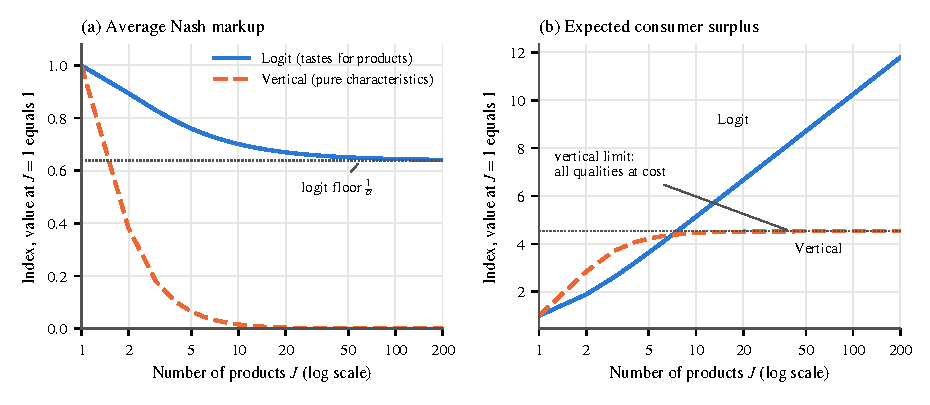
\includegraphics[width=\textwidth]{figures/ch06/clones.pdf}
\caption{Average Nash markup and expected consumer surplus as products are added, in a logit model with identical
products and in a vertical model whose products fill a fixed quality interval. Each product has its own owner. The
logit has $u_{ij} = 2 - p_j + \epsilon_{ij}$, outside good $u_{i0} = \epsilon_{i0}$ and marginal cost $1$. The vertical model
uses Bresnahan's form (\cref{sec:06-bresnahan}), with utility $v\delta_j - p_j$ and $v$ uniform on $[0,1]$. Its
qualities sit at the midpoints of $J$ equal bins of $[1,3]$, marginal cost is $0.05\,e^{\delta}$, and the outside good
has $\delta_0 = p_0 = 0$. Each series is
divided by its value at $J = 1$ because the units of the two models are not comparable. The figure is qualitative.
Computed with \texttt{figures/ch06/src/clones.py}.}
\label{fig:06-clones}
\end{figure}

\Cref{fig:06-clones} computes both models as single-product firms are added. In the logit, the markup falls from
$1.567$ at $J = 1$ to $1.005$ at $J = 200$ and approaches the floor $\frac{1}{\alpha} = 1$. Surplus rises from $0.449$ to
$5.298$ and keeps rising linearly in $\ln J$. In the vertical model, the sales-weighted markup falls from $0.815$ at $J =
1$ to $0.013$ at $J = 10$ and to $0.00003$ at $J = 200$. Surplus converges to $0.752$, the surplus when every quality in
$[1,3]$ is sold at marginal cost.

\subsection{Why the distinction matters}\label{sec:06-eps-matters}

The first implication concerns new goods and price indexes. Retrospective measurement of the gains from new products
goes back to \citet{Trajtenberg1989}, who used a nested logit to value innovations in computed tomography scanners.
Such measurement is also part of constructing ideal price indexes. \citet{BerryPakes2007} note that, according to the Boskin
Commission \citep{BoskinEtAl1996}, failing to measure these gains is the major source of bias in the Consumer Price
Index. A model with tastes for products credits every new variety with a
surplus gain through \eqref{eq:06-logit-gain}, however close it is to existing goods.

\citet[p.~230]{Hausman1997} puts the objection directly. The independence of irrelevant alternatives, he writes,
``typically leads to a vast overestimate of the consumer's surplus from a new good.'' The logit fails to ``incorporate
sufficiently the similarities to existing goods.'' Logit and constant elasticity of substitution demand are positive at every finite price, so the reservation
price at which a new good's demand would vanish is infinite. \citet{Petrin2002} quantifies the role of the shock for
the minivan. His average compensating variation for minivan buyers is \$13,652 with an OLS logit and \$7,414 with an
instrumented logit (1982--84 dollars, his Table~8). It falls to \$3,171 with random coefficients and to \$1,247 when
micro moments are added. The part attributed to the logit error falls from \$95,121 to \$396 across the same columns.
\Cref{ch:newgoods} treats these studies in full.

The second implication concerns market structure. With tastes for products, markups never vanish however many
products crowd the market, so there is always a further incentive to develop products. Market outcomes do not approach
competition as the number of products grows \citep[p.~7]{BerryPakes2007}. A researcher studying a market with hundreds
of products, or the welfare effect of entry, imposes these properties by choosing the model.

\subsection{What the idiosyncratic shock buys}\label{sec:06-eps-advantages}

Models with tastes for products have three practical advantages \citep[pp.~7--8]{BerryPakes2007}. Their choice
probabilities are integrals with simple limits of integration, because conditional on the random coefficients the
logit integral is in closed form \citep{McFadden1981}. Their purchase probabilities are positive at every parameter
value and, under regularity conditions, have smooth derivatives. Their market shares can be inverted to recover the
unobserved characteristics $\xi_j$ as a linear function of parameters and data. Instrumental variables can then handle
the correlation between price and $\xi_j$ \citep{BerryLevinsohnPakes1995}.

Pure characteristics models lose each advantage. The set of tastes for which a product is chosen is a polyhedron whose
shape changes with every parameter value. \citet{FeenstraLevinsohn1995} computed these acceptance regions directly, a
calculation that becomes complicated with several characteristics. Shares are zero whenever a product is dominated,
so the share function has flat regions. The inversion requires new arguments, which \cref{sec:06-purechar} develops.

\subsection{Nesting the two models: the modified BLP model}\label{sec:06-nesting}

A natural idea is to nest the two classes and let the data choose. \citet[eqs.~7--8]{BerryPakes2007} introduce a scale
parameter $\sigma_\epsilon \ge 0$,
\begin{equation}\label{eq:06-nest}
  u_{ij} = f_{ij}(\theta) + \sum_{k=1}^{K} \nu_{ik} X_{jk} + \sigma_\epsilon \epsilon_{ij},
\end{equation}
with $\epsilon_{ij}$ independent standard Gumbel. The model with tastes for products is the case $\sigma_\epsilon = 1$,
and the pure characteristics model is the case $\sigma_\epsilon = 0$. For $\sigma_\epsilon > 0$ define $\mu_\epsilon =
\frac{1}{\sigma_\epsilon}$ and multiply all utilities by $\mu_\epsilon$. This leaves choices unchanged. If $F(\nu)$ is the
distribution of $\nu = (\nu_1, \dots, \nu_K)$, the logit formula gives (their eq.~9)
\begin{equation}\label{eq:06-modblp}
  P_{ij}(\theta, \mu_\epsilon) = \int
  \frac{\exp\bigl(\mu_\epsilon\bigl[f_{ij}(\theta) + \sum_{k} \nu_k X_{jk}\bigr]\bigr)}
       {\sum_{q} \exp\bigl(\mu_\epsilon\bigl[f_{iq}(\theta) + \sum_{k} \nu_k X_{qk}\bigr]\bigr)} \,\dd F(\nu).
\end{equation}
We call \eqref{eq:06-modblp} the \emph{modified BLP model}. Formula \eqref{eq:06-modblp} needs $\mu_\epsilon < \infty$,
so no value of $\mu_\epsilon$ reproduces the pure characteristics model exactly. It is reached only as a limit.

\begin{proposition}[Pure characteristics as a limit]\label{prop:06-limit}
Let $U_{ij}(\nu) = f_{ij}(\theta) + \sum_k \nu_k X_{jk}$ and let
\begin{equation*}
  P^{pc}_{ij}(\theta) = \int \indic\bigl\{U_{ij}(\nu) > U_{iq}(\nu) \text{ for all } q \ne j\bigr\}\,\dd F(\nu)
\end{equation*}
be the pure characteristics choice probability. Suppose ties have probability zero, that is, $F$ assigns probability
zero to the set of $\nu$ with $U_{ij}(\nu) = U_{iq}(\nu)$ for some $q \ne j$. Then $P_{ij}(\theta, \mu_\epsilon) \to
P^{pc}_{ij}(\theta)$ as $\mu_\epsilon \to \infty$.
\end{proposition}

\begin{proof}
Fix $\nu$ outside the tie set and let $m$ be the unique maximizer of $U_{iq}(\nu)$ over $q$. Divide the numerator and
denominator of the integrand by the numerator to obtain
\begin{equation*}
  \frac{1}{1 + \sum_{q \ne j} \exp\bigl(\mu_\epsilon [U_{iq}(\nu) - U_{ij}(\nu)]\bigr)} .
\end{equation*}
If $j = m$, every exponent is negative and each exponential converges to zero, so the integrand converges to one. If
$j \ne m$, the exponent for $q = m$ is positive and that exponential diverges, so the integrand converges to zero. The
integrand therefore converges to $\indic\{j = m\}$ for $F$-almost every $\nu$. It lies in $[0,1]$, and the constant one
is integrable against the probability measure $F$. The dominated convergence theorem gives the result.
\end{proof}

\citet[footnote~9]{BerryPakes2007} add that a covering argument makes the convergence uniform in $\theta$. One might
hope that estimating $\mu_\epsilon$ along with the other parameters would deliver a large estimate whenever the pure
characteristics model generated the data. \citet[p.~9]{BerryPakes2007} give four reasons to doubt it.
\begin{enumerate}
\item Consistency proofs assume that the true parameter lies in a compact set. One would therefore have to prove
consistency for $\sigma_\epsilon = \frac{1}{\mu_\epsilon}$ on an interval that contains zero. The predicted shares are
undefined at $\sigma_\epsilon = 0$. The objective is then not a continuous function on a compact parameter set that
contains the truth, and the uniform convergence that standard proofs require fails at that boundary.
\item A good approximation needs a small $\sigma_\epsilon$, that is, a large $\mu_\epsilon$. For large $\mu_\epsilon$ the
computer cannot evaluate the exponentials in \eqref{eq:06-modblp}.
\item If $\sigma_\epsilon$ is known to be zero, an estimator that imposes it should estimate the other parameters more
precisely. With market-level data this efficiency gain can matter.
\item To learn whether these problems matter in a given application, one needs an estimator that does not rely on the
approximation \eqref{eq:06-modblp}.
\end{enumerate}
A test of $\sigma_\epsilon = 0$ faces a further, standard difficulty. The null hypothesis lies on the boundary of the
parameter space, where likelihood-ratio and Wald statistics have nonstandard limiting distributions.

\begin{remark}[The two models as bounds]\label{rem:06-bounding}
Real products differ in more than one unobserved characteristic. A pure characteristics model with as many unobserved
characteristics as products contains the model with tastes for products as a special case, by
\eqref{eq:06-dummies}. The pure characteristics model with a single unobserved characteristic and the model with
tastes for products are therefore opposite extremes. \citet[p.~12]{BerryPakes2007} suggest that the two might bound the
effects of unobserved product heterogeneity. Models with several unobserved characteristics are hard to estimate
from market data, although panel data on repeated choices of the same consumers can identify them
\citep{GoettlerShachar2001}.
\end{remark}

\section{Case study: estimating the pure characteristics model}\label{sec:06-purechar}

\citet{BerryPakes2007} turn the pure characteristics model, long used in theory, into an estimable model for market
data. Their paper has no field data. It develops the econometric machinery and then uses Monte Carlo experiments to
compare the pure characteristics model with models that have tastes for products. We follow the order of a case study,
with the simulated designs in the place of a data set.

\subsection{The question}\label{sec:06-bp-question}

The paper asks three questions. Can the pure characteristics model be estimated from market-level data on prices,
quantities and characteristics? How much computation does that take? When do models with tastes for products, possibly
with an estimated scale $\mu_\epsilon$, reproduce the implications of the pure characteristics model for elasticities and
for welfare? The questions matter because welfare analysis of new products extrapolates beyond observed prices. As
\cref{sec:06-epsilon} showed, the two classes of models extrapolate very differently.

\subsection{Model and normalizations}\label{sec:06-bp-model}

Utility of consumer $i$ from product $j = 0, 1, \dots, J$ is (their eq.~10)
\begin{equation}\label{eq:06-bp-u10}
  u_{ij} = x_j \beta_i - \alpha_i p_j + \lambda_i \xi_j ,
\end{equation}
with $\beta_{ik} = \beta_k + \nu_{ik}$, $\alpha_i = \alpha + \nu_{ip} > 0$ and $\lambda_i > 0$. Here $\beta_k$ is the mean
marginal utility of characteristic $k$ and $\nu_{ik}$ is consumer $i$'s deviation from it. Two assumptions are built into
\eqref{eq:06-bp-u10}.

\begin{assumption}[Berry and Pakes, A1 and A2]\label{ass:06-bp}
(A1) There is a single unobserved product characteristic, so $X_j = (x_j, \xi_j) \in \R^K \times \R$. (A2) The unobserved
characteristic is vertical: every consumer prefers more of it.
\end{assumption}

Utility is identified only up to a consumer-specific increasing affine transformation (\cref{prop:06-normalization}).
Berry and Pakes use both degrees of freedom. They subtract $u_{i0}$ from every utility, so the outside option has utility
zero and every characteristic is measured relative to the outside option. They then divide by $\lambda_i$, so the
coefficient on $\xi$ equals one for every consumer. After relabeling the rescaled coefficients, the model is (their
eq.~11)
\begin{equation}\label{eq:06-bp-u11}
  u_{ij} = x_j \beta_i - \alpha_i p_j + \xi_j , \qquad u_{i0} = 0 .
\end{equation}
This is the model of \citet{BerryLevinsohnPakes1995} without the shock $\epsilon_{ij}$. Units remain free. Multiplying
every $\xi_j$, $\beta_i$ and $\alpha_i$ by the same positive constant changes no choice (their footnote~12). Berry and
Pakes set the mean of $\alpha_i$ to one, so utility and $\xi$ are measured in units of the mean price coefficient.

Two interpretive points follow from the normalizations. First, $\xi_j$ measures the unobserved quality of product $j$
relative to that of the outside option (their footnote~11). A rise in average $\xi$ over time may therefore reflect
better products or a worse outside option, which matters for price indexes \citep{PakesBerryLevinsohn1993}. Second,
$\xi_j$ often stands for the combined effect of many minor characteristics (their footnote~4). If consumers differ in
their relative tastes for several unobserved characteristics, \eqref{eq:06-bp-u11} is misspecified.

\subsection{Computing market shares}\label{sec:06-bp-shares}

\casehead{The vertical building block}
Start with the vertical model $u_{ij} = \delta_j - \alpha_i p_j$, where $\delta_j = x_j\beta + \xi_j$ is quality (their
eqs.~12--13). It is the model of \cref{sec:06-vertical} with the price coefficient $\alpha_i$ in the role of the price
sensitivity $\nu_i$. Order the goods by increasing price. \Cref{sec:06-vcutoffs} showed that consumer $i$ buys $j$ if and
only if $\underline\nu_j(\delta, p) < \alpha_i < \bar\nu_j(\delta, p)$, with the general cutoffs
\eqref{eq:06-bp-cutoffs} (their eqs.~14--16). If $F$ is the distribution of $\alpha_i$, the share of product $j$ is
\eqref{eq:06-bp-share} (their eq.~17). We write it as $s_j(x, p, \xi; \theta, F)$ to show its dependence on the data and
on the unknown parameters $\theta$. Any parameter vector that puts a product below the quality-price frontier predicts a zero
share for it. A model with tastes for products never predicts a zero share.

\casehead{Extension to $K$ dimensions}
In \eqref{eq:06-bp-u11} the coefficients on $x$ vary across consumers. Conditional on $\beta_i = \beta$, however, the model
is again vertical in $\alpha_i$, with qualities $\delta_j(\beta) = x_j \beta + \xi_j$ that depend on the draw. Compute the
cutoffs $\bar\nu_j(\beta)$ and $\underline\nu_j(\beta)$ from \eqref{eq:06-bp-cutoffs} with $\delta_j(\beta)$ in place of
$\delta_j$, and integrate over $\beta$ (their eq.~18):
\begin{equation}\label{eq:06-bp-share18}
  s_j(x, p, \xi; \theta, F, G) = \int \bigl[F(\bar\nu_j(\beta) \mid \beta) - F(\underline\nu_j(\beta) \mid \beta)\bigr]\,
  \indic\{\bar\nu_j(\beta) > \underline\nu_j(\beta)\}\, \dd G(\beta) .
\end{equation}
Here $F(\cdot \mid \beta)$ is the distribution of $\alpha_i$ given $\beta_i = \beta$ and $G$ is the distribution of
$\beta_i$. The pure characteristics share function is a mixture of vertical-model share functions. The conditioning
argument avoids computing the region of $(\beta, \alpha)$ space in which a consumer chooses $j$, the route taken by
\citet{FeenstraLevinsohn1995}. The integral over $\beta$ has no closed form, so it is simulated \citep{Pakes1986}. With
$ns$ draws $\beta_1, \dots, \beta_{ns}$ from $G$ and their empirical distribution $G_{ns}$ (their eqs.~19--20),
\begin{equation}\label{eq:06-bp-share20}
  s_j(x, p, \xi; \theta, F, G_{ns}) = \frac{1}{ns} \sum_{r=1}^{ns}
  \bigl[F(\bar\nu_j(\beta_r) \mid \beta_r) - F(\underline\nu_j(\beta_r) \mid \beta_r)\bigr]\,
  \indic\{\bar\nu_j(\beta_r) > \underline\nu_j(\beta_r)\} .
\end{equation}
Berry and Pakes note that if $F$ has a density that is differentiable in the parameters, the simulated share function is
continuously differentiable in the parameters. The simulation adds error to the computed shares, as in
\citet{BerryLevinsohnPakes1995}.

The comparison with the random coefficients logit is instructive. There the first step integrates out $\epsilon_{ij}$
analytically conditional on $\beta_i$, which yields the logit formula. Here the first step integrates out $\alpha_i$
analytically conditional on $\beta_i$, which yields the vertical formula. Both models simulate the remaining
integral. A practical version of \eqref{eq:06-bp-share20} proceeds as follows (their footnote~15).
\begin{enumerate}
\item Draw $\beta_1, \dots, \beta_{ns}$ from $G$ once, and keep the draws fixed across parameter values so that the
objective function is smooth in the parameters.
\item For each draw $r$, compute $\delta_j(\beta_r) = x_j \beta_r + \xi_j$ for $j = 1, \dots, J$, with $\delta_0 = p_0 = 0$.
\item Sort the products by price and drop those that are dominated for this draw, using the frontier algorithm that
follows \cref{prop:06-frontier}. The survivors have decreasing adjacent cutoffs.
\item For each survivor compute $F(\bar\nu_j \mid \beta_r) - F(\bar\nu_{j+1} \mid \beta_r)$ with cutoffs between adjacent
survivors. Assign zero to the dropped products.
\item Average the conditional shares over the $ns$ draws.
\end{enumerate}
In the Monte Carlo design of \cref{sec:06-bp-design}, $\ln\alpha_i = \sigma_p \nu_{ip}$ with $\nu_{ip}$ standard normal and
independent of $\beta_i$. Step 4 then uses $F(a \mid \beta) = \Phi\bigl(\frac{\ln a}{\sigma_p}\bigr)$ for $a > 0$, with $\Phi$
the standard normal distribution function.

\subsection{Existence and uniqueness of the inverse}\label{sec:06-bp-inverse}

Estimation follows the three steps of \citet{BerryLevinsohnPakes1995}. For each parameter vector one recovers the
unobserved characteristics from the observed shares, computes them with an algorithm, and then chooses the parameters
that best satisfy moment conditions on $\xi$. The first step requires that the share equations have exactly one
solution.

Fix $(x, p, \theta, F, G)$ and write $\sigma_j(\xi_0, \xi)$, $j = 0, 1, \dots, J$, for the share of good $j$ as a function of
the unobserved characteristics of all goods, the outside good included. Let $s^o$ be the observed share vector, assumed
to lie in the interior of the unit simplex, so that every share is strictly between zero and one. With the normalization
$\xi_0 = 0$, we seek $\xi \in \R^J$ such that (their eq.~21)
\begin{equation}\label{eq:06-bp-system}
  \sigma(0, \xi) = s^o .
\end{equation}
For good $j \ge 1$ define the \emph{element-by-element inverse} $r_j(\xi_{-j})$ as the value of $\xi_j$ that matches good
$j$'s share when the other inside goods are held at $\xi_{-j}$ (their eq.~23):
\begin{equation}\label{eq:06-bp-r}
  \sigma_j\bigl(0, r_j(\xi_{-j}), \xi_{-j}\bigr) = s^o_j .
\end{equation}
Stack the inverses into $r(\xi) = (r_1(\xi_{-1}), \dots, r_J(\xi_{-J}))$, a map from $\R^J$ to $\R^J$. A vector $\xi$ solves
\eqref{eq:06-bp-system} if and only if it is a fixed point (their eq.~24)
\begin{equation}\label{eq:06-bp-fixedpoint}
  \xi = r(\xi) .
\end{equation}
Indeed, a fixed point matches every inside share, and the outside share then matches because shares sum to one.

\begin{theorem}[Berry and Pakes 2007, Theorem~1]\label{thm:06-bp-inverse}
Suppose the share function $\sigma$ has the following properties.\footnote{\citet{BerryPakes2007} state monotonicity in
weak form and the substitutes condition as the pair of inequalities in their eqs.~25--26. We add strict monotonicity in
own $\xi$ on the interior, which makes the element-by-element inverse single valued. We also state the substitutes
condition in the form that the proof uses. \citet{BerryGandhiHaile2013} generalize conditions of this type under the
name ``connected substitutes''.}
\begin{enumerate}[label=(\arabic*)]
\item \emph{Monotonicity.} Each $\sigma_j$, $j = 0, \dots, J$, is continuous, nondecreasing in its own $\xi_j$ and
nonincreasing in every other component. It is strictly increasing in $\xi_j$ at any point where $0 < \sigma_j < 1$. For
fixed values of the other components, $\sigma_j \to 0$ as $\xi_j \to -\infty$ and $\sigma_j \to 1$ as $\xi_j \to \infty$.
\item \emph{Linearity of utility in $\xi$.} Raising $\xi$ for every good, the outside good included, by the same amount
changes no share: $\sigma(\xi_0 + c, \xi + c\mathbf{1}) = \sigma(\xi_0, \xi)$ for every $c \in \R$.
\item \emph{Substitutes with some other good.} Let $(\xi_0, \xi)$ give interior shares. Let $(\tilde\xi_0, \tilde\xi) \ge
(\xi_0, \xi)$ componentwise, with equality exactly on a nonempty proper subset $I$ of $\{0, 1, \dots, J\}$. Then
$\sigma_j(\tilde\xi_0, \tilde\xi) < \sigma_j(\xi_0, \xi)$ for at least one $j \in I$.
\end{enumerate}
Then for every $s^o$ in the interior of the unit simplex, \eqref{eq:06-bp-system} has exactly one solution $\xi \in \R^J$.
Moreover, $r$ is a weak contraction in the sup norm: $\lVert r(\xi') - r(\xi) \rVert_\infty \le \lVert \xi' - \xi
\rVert_\infty$.
\end{theorem}

Condition (3) says that when the unobserved characteristics of some goods rise, at least one good whose characteristic
did not rise loses share strictly. The proof has five steps. Steps 3 and 4 follow \citet[eqs.~27--31]{BerryPakes2007}.
They attribute existence to the argument in \citet{Berry1994}. Step 5 gives a self-contained existence argument.
Throughout we write the arguments of $\sigma_j$ in the order (outside good, own, other inside goods) when it helps.

\begin{proof}
\emph{Step 1: $r$ is well defined and continuous.} Fix $j$ and $\xi_{-j}$, and let $g(a) = \sigma_j(0, a, \xi_{-j})$. By
condition (1), $g$ is continuous with limits $0$ and $1$. Since $0 < s^o_j < 1$, the intermediate value theorem gives a
solution of $g(a) = s^o_j$. Two solutions $a < a'$ would make $g$ constant at the interior value $s^o_j$ on $[a, a']$,
which strict monotonicity rules out. For continuity of $r_j$, take $h > 0$. Strict monotonicity gives $g(r_j + h) > s^o_j > g(r_j - h)$. By
continuity of $\sigma_j$ in $\xi_{-j}$, both strict inequalities survive small changes in $\xi_{-j}$, which keeps the
solution within $h$ of $r_j$.

\emph{Step 2: $r$ is monotone.} Let $\xi \le \xi'$ and suppose $r_j(\xi'_{-j}) < r_j(\xi_{-j})$ for some $j$. Raising the
rivals from $\xi_{-j}$ to $\xi'_{-j}$ weakly lowers $j$'s share, so
\begin{equation*}
  s^o_j = \sigma_j\bigl(0, r_j(\xi'_{-j}), \xi'_{-j}\bigr) \le \sigma_j\bigl(0, r_j(\xi_{-j}), \xi'_{-j}\bigr)
  \le \sigma_j\bigl(0, r_j(\xi_{-j}), \xi_{-j}\bigr) = s^o_j .
\end{equation*}
The first inequality uses own monotonicity. Both inequalities hold with equality, so $\sigma_j(0, \cdot, \xi'_{-j})$ is
constant at $s^o_j$ on an interval, which contradicts strict monotonicity. Hence $r(\xi) \le r(\xi')$.

\emph{Step 3: $r$ is a weak contraction.} Take $\xi, \xi' \in \R^J$ with $d = \lVert \xi - \xi' \rVert_\infty$, and write
$r_j = r_j(\xi_{-j})$ and $r'_j = r_j(\xi'_{-j})$. By the definition of $r_j$ and linearity with $c = d$,
\begin{equation}\label{eq:06-bp-p27}
  \sigma_j\bigl(d, r_j + d, \xi_{-j} + d\bigr) = \sigma_j\bigl(0, r_j, \xi_{-j}\bigr) = s^o_j .
\end{equation}
Now $\xi'_{-j} \le \xi_{-j} + d$ and $0 < d$. Lowering the rivals' characteristics from $(d, \xi_{-j} + d)$ to $(0,
\xi'_{-j})$ weakly raises $j$'s share, so
\begin{equation}\label{eq:06-bp-p28}
  \sigma_j\bigl(0, r_j + d, \xi'_{-j}\bigr) \ge s^o_j .
\end{equation}
Suppose $r'_j > r_j + d$. Then own monotonicity and \eqref{eq:06-bp-p28} give
\begin{equation*}
  s^o_j = \sigma_j\bigl(0, r'_j, \xi'_{-j}\bigr) \ge \sigma_j\bigl(0, r_j + d, \xi'_{-j}\bigr) \ge s^o_j ,
\end{equation*}
so $\sigma_j(0, \cdot, \xi'_{-j})$ would be constant at $s^o_j$ on $[r_j + d, r'_j]$. This contradicts strict
monotonicity, so $r'_j \le r_j + d$. The same argument with $c = -d$ gives $r'_j \ge r_j - d$. Hence $|r'_j - r_j| \le d$
for every $j$, which is the weak contraction property.

\emph{Step 4: uniqueness.} Suppose $\xi \ne \xi'$ both solve \eqref{eq:06-bp-system}. Exchanging their names if
necessary, $\bar c = \max_k (\xi_k - \xi'_k) > 0$. Let $I = \{k : \xi_k - \xi'_k = \bar c\}$, a nonempty set of inside goods.
Define $\tilde\xi = \xi' + \bar c\mathbf{1}$ and $\tilde\xi_0 = \bar c$. By linearity,
\begin{equation*}
  \sigma(\tilde\xi_0, \tilde\xi) = \sigma(0, \xi') = s^o .
\end{equation*}
Compare $(\tilde\xi_0, \tilde\xi)$ with $(0, \xi)$. For each inside good, $\tilde\xi_k - \xi_k = \bar c - (\xi_k - \xi'_k) \ge
0$, with equality exactly for $k \in I$. For the outside good, $\tilde\xi_0 - 0 = \bar c > 0$. So $(\tilde\xi_0, \tilde\xi) \ge
(0, \xi)$ with equality exactly on $I$, a nonempty proper subset of $\{0, \dots, J\}$. Shares at $(0, \xi)$ equal $s^o$ and are
interior. Condition (3) then yields a good $j \in I$ with $\sigma_j(\tilde\xi_0, \tilde\xi) < \sigma_j(0, \xi) = s^o_j$. But
$\sigma_j(\tilde\xi_0, \tilde\xi) = s^o_j$, a contradiction.

\emph{Step 5: existence.} We first find a vector $\xi^{(0)}$ with $r(\xi^{(0)}) \ge \xi^{(0)}$. By linearity,
$\sigma(0, a\mathbf{1}) = \sigma(-a, \mathbf{0})$. As $a \to -\infty$, the outside good's own characteristic $-a$ goes to
infinity, so by condition (1) its share goes to one and every inside share goes to zero. Choose $a$ with $\sigma_j(0,
a\mathbf{1}) < s^o_j$ for all $j \ge 1$. At own value $a$ and rivals at $a$, good $j$ falls short of its target, so own
monotonicity gives $r_j(a\mathbf{1}_{-j}) > a$. Set $\xi^{(0)} = a\mathbf{1}$ and iterate $\xi^{(n+1)} = r(\xi^{(n)})$. By
Step 2 and induction, the sequence is nondecreasing.

Next, the sequence is bounded. Because it is nondecreasing, it can be unbounded only if some component
diverges to infinity. Since $\xi^{(n)}_j \le r_j(\xi^{(n)}_{-j})$ and $\sigma_j$ increases in own $\xi_j$, every
inside share satisfies $\sigma_j(0, \xi^{(n)}) \le s^o_j$. Shares sum to one, so $\sigma_0(0, \xi^{(n)}) \ge s^o_0 > 0$.
Suppose component $\xi^{(n)}_k$ diverged. Because the other components are at least $\xi^{(0)}_{-k}$ and
$\sigma_0$ is nonincreasing in inside characteristics,
\begin{equation*}
  \sigma_0\bigl(0, \xi^{(n)}\bigr) \le \sigma_0\bigl(0, \xi^{(n)}_k, \xi^{(0)}_{-k}\bigr)
  \le 1 - \sigma_k\bigl(0, \xi^{(n)}_k, \xi^{(0)}_{-k}\bigr) \to 0 ,
\end{equation*}
by the limit in condition (1). This contradicts $\sigma_0 \ge s^o_0$. A bounded nondecreasing sequence converges, say to
$\xi^*$. By continuity of $r$, $\xi^* = \lim r(\xi^{(n)}) = r(\xi^*)$, so $\xi^*$ solves \eqref{eq:06-bp-system}.
\end{proof}

\begin{remark}[The conditions in the pure characteristics model]\label{rem:06-bp-conditions}
\citet[Comment~1]{BerryPakes2007} observe that the conditions hold for any finite $\theta$ as long as $F(\cdot \mid \beta)$
has a positive density. The distribution $G$ need not have a density, so the simulated $G_{ns}$ of
\eqref{eq:06-bp-share20} is allowed. Linearity holds by construction in \eqref{eq:06-bp-u11}, and their Comment~2 notes
that any model that is linear in $\xi$ alone would share the result. Condition (3) can be checked draw by draw.
Conditional on $\beta$, the undominated goods form a chain ordered by price, and each good on the chain competes with its
neighbors. The outside good is always on the chain. If the chain contains goods both inside and outside $I$, some
adjacent pair has one member in each. Raising the characteristic of the member outside $I$ strictly lowers the
conditional share of its neighbor in $I$, because $F$ has a positive density. Interior aggregate shares ensure that
such draws have positive probability.
\end{remark}

Steps 3 to 5 are constructive. The iteration in Step 5 is the element-by-element inverse started from a low point. It
converges monotonically, but the argument gives no rate. The weak contraction property gives no rate either, because its
modulus may equal one. \citet{BerryPakes2007} report that they could not prove a modulus below one. This is the main
computational difference from the logit-based contraction of \citet{BerryLevinsohnPakes1995}, which converges at a
geometric rate.

\subsection{Computing the inverse}\label{sec:06-bp-compute}

Berry and Pakes offer three methods, because each fails in some of their experiments.

\casehead{The modified BLP contraction}
Apply the BLP contraction of \cref{ch:blp} to the modified BLP model \eqref{eq:06-modblp} with a large fixed
$\mu_\epsilon$. Since the logit part of \eqref{eq:06-modblp} depends on mean utility only through $\mu_\epsilon\delta$, the
iteration on mean utilities reads
\begin{equation}\label{eq:06-modblp-contraction}
  \delta^{(h+1)} = \delta^{(h)} + \frac{1}{\mu_\epsilon}\bigl[\ln s^o - \ln s(\delta^{(h)}; \mu_\epsilon)\bigr] .
\end{equation}
The method is fast. It is inaccurate when $\mu_\epsilon$ cannot be set high enough, and numerical overflow limits how
high it can go.

\casehead{The element-by-element inverse}
Start from a candidate vector. For each product $j$, hold the other products at their current values and solve the
one-dimensional monotone equation \eqref{eq:06-bp-r} for $\xi_j$. Update all products and repeat until predicted shares
match observed shares. By \cref{thm:06-bp-inverse} each pass is a weak contraction. In practice the method sometimes
makes large gains in the first iterations and then nearly stops. If predicted shares are then positive, Newton steps can
finish the job.

\casehead{The homotopy}
A homotopy deforms a problem with a known solution into the problem of interest. Berry and Pakes use the fixed-point
homotopy (their eq.~32)
\begin{equation}\label{eq:06-homotopy}
  h(\xi, t, \xi_0) = (1 - t)(\xi - \xi_0) + t\bigl(\xi - r(\xi)\bigr), \qquad t \in [0, 1],
\end{equation}
where $\xi_0$ is a starting guess, for example the output of another method. Let $\xi(t)$ solve $h(\xi, t, \xi_0) = 0$.
At $t = 0$ the solution is $\xi_0$, and at $t = 1$ it is the fixed point \eqref{eq:06-bp-fixedpoint}. Rearranging $h = 0$
gives (their eq.~33)
\begin{equation}\label{eq:06-homotopy33}
  \xi(t) = (1 - t)\,\xi_0 + t\, r\bigl(\xi(t)\bigr) .
\end{equation}

\begin{proposition}[Convergence of the homotopy]\label{prop:06-homotopy}
Under the conditions of \cref{thm:06-bp-inverse}, let $\xi^*$ be the unique solution of \eqref{eq:06-bp-system}.
\begin{enumerate}[label=(\roman*)]
\item For each $t \in [0, 1)$, the map $\Phi_t(\xi) = (1 - t)\xi_0 + t\, r(\xi)$ is a contraction with modulus at most $t$.
Hence $\xi(t)$ exists, is unique, and is the limit of the recursion $\xi \mapsto (1-t)\xi_0 + t\,r(\xi)$ (their eq.~34)
from any starting point.
\item $\lVert \xi(t) - \xi^* \rVert_\infty \le \lVert \xi_0 - \xi^* \rVert_\infty$ for every $t \in [0,1)$, and $\xi(t) \to
\xi^*$ as $t \to 1$.
\end{enumerate}
\end{proposition}

\begin{proof}
For (i), $\lVert \Phi_t(\xi) - \Phi_t(\xi') \rVert_\infty = t \lVert r(\xi) - r(\xi') \rVert_\infty \le t \lVert \xi - \xi'
\rVert_\infty$ by the weak contraction property. The contraction mapping theorem (\cref{app:math}) gives the rest.

For (ii), subtract $\xi^* = (1 - t)\xi^* + t\, r(\xi^*)$ from \eqref{eq:06-homotopy33}:
\begin{equation*}
  \xi(t) - \xi^* = (1 - t)(\xi_0 - \xi^*) + t\bigl[r(\xi(t)) - r(\xi^*)\bigr] .
\end{equation*}
Taking norms and using the weak contraction property,
\begin{equation*}
  \lVert \xi(t) - \xi^* \rVert_\infty \le (1 - t)\lVert \xi_0 - \xi^* \rVert_\infty + t \lVert \xi(t) - \xi^* \rVert_\infty .
\end{equation*}
Collecting terms and dividing by $1 - t > 0$ gives the bound. The path is therefore bounded. Take any sequence $t_n \to 1$
along which $\xi(t_n)$ converges, say to $\hat\xi$. Passing to the limit in \eqref{eq:06-homotopy33} and using continuity of
$r$ gives $\hat\xi = r(\hat\xi)$. By uniqueness $\hat\xi = \xi^*$. Every convergent subsequence has the same limit, so
$\xi(t) \to \xi^*$.
\end{proof}

The modulus $t$ explains the practical behavior. Each tenfold reduction in the error of the recursion takes about
$\frac{\ln 10}{-\ln t}$ iterations. That is about 229 iterations at $t = 0.99$, 459 at $t = 0.995$ and 1,150 at
$t = 0.998$. Berry and Pakes start at $t = 0.99$ and move $t$ toward one slowly, solving for each new $\xi(t)$ by Newton's
method when the recursion becomes slow. They find that the homotopy gets much closer to the solution than the
element-by-element inverse before it slows down.

What the paper calls the ``homotopy'' method is an integrated routine that combines the three methods.
\begin{enumerate}
\item Run the modified BLP contraction \eqref{eq:06-modblp-contraction} with a high $\mu_\epsilon$, lowering
$\mu_\epsilon$ if numerical errors arise.
\item If needed, switch to the element-by-element inverse, with periodic Newton steps when possible.
\item If that does not converge quickly, use the homotopy recursion. For small problems, push $t$ to one or very near it.
For large problems, use only a few values such as $t = 0.99$, $0.995$ and $0.998$.
\end{enumerate}

\subsection{Simulation error and limit theory}\label{sec:06-bp-simerror}

\citet{BerryLintonPakes2004} derive limit theorems as the number of products $J$ grows, for models with and without
tastes for products. The two classes behave very differently, and the difference has computational consequences.

In the plain logit no simulation is needed, but observed shares contain sampling error from a finite sample of
consumers. The inversion is analytic (their eqs.~35--36),
\begin{equation}\label{eq:06-logit-inv-sens}
  \xi_j = \ln s_j - \ln s_0 - x_j \beta , \qquad \frac{\partial \xi_j}{\partial s_j} = \frac{1}{s_j} .
\end{equation}
With many products most shares are small, so the recovered $\xi_j$ are very sensitive to any error in $s_j$.
\citet{BerryLintonPakes2004} show that simulation error causes the same problem in the random coefficients logit. A
back-of-the-envelope calculation shows the orders of magnitude. If $s_j$ is estimated from $n$ independent draws, its
variance is about $\frac{s_j(1 - s_j)}{n}$. The delta method then gives
\begin{equation*}
  \Var(\ln \hat s_j) \approx \frac{1}{s_j^2}\cdot\frac{s_j(1 - s_j)}{n} = \frac{1 - s_j}{n s_j} .
\end{equation*}
With $s_j$ of order $\frac{1}{J}$, the standard deviation of the error in $\xi_j$ is of order $\sqrt{\frac{J}{n}}$. It grows
with the number of products unless $n$ grows faster than $J$.

The pure characteristics model behaves in the opposite way. As products crowd the space, competition becomes local and
fierce, so $\frac{\partial s_j}{\partial \xi_j}$ is large and the inverse map is insensitive to share errors. The
vertical model makes this concrete. By \cref{prop:06-vinversion}, $\delta_j = \sum_{m \le j} (p_m - p_{m-1})
F^{-1}(S_m)$, where $S_m = \sum_{k \ge m} s_k$ is a cumulative share. A cumulative share estimated from $n$ draws has
variance at most $\frac{1}{4n}$, whatever $J$. The weights $\frac{p_m - p_{m-1}}{f(F^{-1}(S_m))}$ translate errors
in $S_m$ into errors in $\delta_j$. Their sum is bounded when prices lie in a bounded interval and the density $f$ is
bounded away from zero there. The error in each $\delta_j$ is then of order $\frac{1}{\sqrt n}$, independent of $J$.

The formal results preserve this ranking, with higher required rates than the heuristic suggests.
\citet{BerryLintonPakes2004} derive conditions for asymptotic normality of the parameter estimates. The number of
simulation draws must grow at rate $J$ in the vertical model and at rate $J^2$ in logit-type models.
\citet[p.~23]{BerryPakes2007} report the Monte Carlo results of that paper. About fifty draws suffice for the limit
distribution to describe the vertical model with up to two hundred products. The logit with one
hundred products requires over two thousand draws.

Two forces therefore pull in opposite directions \citep[pp.~23--24]{BerryPakes2007}. The required number of draws grows
like $J^2$ with tastes for products and like $J$ without them, which favors the pure characteristics model. The BLP
contraction converges geometrically, while no rate is known for the pure characteristics inverse, which favors the
model with tastes for products. Which force dominates depends on the number of products and on how often the inverse
must be computed, which grows with the number of parameters.

\subsection{Estimator, instruments and identification}\label{sec:06-bp-estimator}

Write mean quality as $\delta_j = x_j\beta + \xi_j$ and split the parameters into the linear parameters $\theta_1 = \beta$
and the nonlinear parameters $\theta_2$ that govern the distribution of $(\beta_i - \beta, \alpha_i)$. For each $\theta_2$,
\cref{thm:06-bp-inverse} delivers a unique $\delta(\theta_2)$ that matches the observed shares, computed by the methods of
\cref{sec:06-bp-compute}. The structural error is $\xi_j(\theta) = \delta_j(\theta_2) - x_j\beta$. With instruments $z_j$
satisfying $\E[\xi_j z_j] = 0$, the GMM estimator solves
\begin{equation}\label{eq:06-bp-gmm}
  \hat\theta = \argmin_{\theta} \; \xi(\theta)^\top Z\, W\, Z^\top \xi(\theta),
\end{equation}
where $Z$ stacks the instruments and $W$ is a weighting matrix. The linear parameters can be concentrated out by
instrumental variables regression of $\delta(\theta_2)$ on $x$, exactly as in \cref{ch:blp}.

Price is correlated with $\xi$ in any equilibrium model, so the instruments must exclude it. The small Monte Carlo design
uses five instruments. They are a constant, $x$, $x^2$, the market mean of $x$ and the distance from each product to its
nearest neighbor in $x$. These functions of the characteristics of rival products shift each product's competitive
environment, and so its price and share, without entering its own utility. The distance to the nearest neighbor suits
the pure characteristics model, where substitution is local. An approximation to optimal instruments had little effect
(their footnote~17). The large design uses a constant and $x$, each interacted with market dummies. Berry and Pakes
attribute their success to the requirement that one utility model fit three markets whose product sets differ sharply.

\subsection{The Monte Carlo designs}\label{sec:06-bp-design}

Data are drawn from the model (their eqs.~37--39)
\begin{equation}\label{eq:06-bp-mc}
  u_{ij} = \delta_j + \sigma_x \nu_{ix} x_j - \alpha_i p_j , \qquad
  \ln \alpha_i = \sigma_p \nu_{ip} , \qquad
  \delta_j = \beta_0 + \beta_x x_j + \xi_j ,
\end{equation}
with $(\nu_{ix}, \nu_{ip})$ independent standard normal. The true values are $\sigma_x = 1$, $\sigma_p = 1$, $\beta_0 = 2$ and
$\beta_x = 1$. The price coefficient is lognormal with $\E[\ln \alpha_i] = 0$. This fixes the median of $\alpha_i$ at
one. Its mean is $e^{\frac{\sigma_p^2}{2}} \approx 1.65$ at the true $\sigma_p = 1$. The design therefore normalizes the
median of the price coefficient, while their text describes a normalization of the mean
\citep[p.~11]{BerryPakes2007}.

The characteristic $x$ equals twice a firm-specific uniform $(0,1)$ draw plus one half of a uniform $(0,1)$ draw common to
all firms in the market, which correlates characteristics within a market. Its variance is $\frac{4}{12} + \frac{1}{4}
\cdot \frac{1}{12} = \frac{17}{48} \approx 0.354$. In the base design $\xi_j$ is uniform on $(-\frac{1}{2}, \frac{1}{2})$,
with variance $\frac{1}{12} \approx 0.083$. A second design uses $\xi_j$ uniform on $(-1.5, 1.5)$, with variance $0.75$, which
exceeds the variance of $x$. Price is a convex function of quality, $p_j = \frac{e^{\delta_j}}{20}$. Equivalently, $\delta_j
= \ln(20 p_j)$ is strictly concave in price. In the vertical case this makes the cutoffs strictly decreasing, so every
product sells (\cref{prop:06-frontier}). Since price depends on $\delta_j$ and hence on $\xi_j$, price is endogenous by
construction. Observed shares come from the choices of 5,000 simulated consumers at the true parameters. Prices come
from this formula, and no pricing game is solved, so the design does not need a price equilibrium to exist.
Dividing utility by $\alpha_i$ puts it in the linear form of assumption A1 of \citet{CaplinNalebuff1991}, with type
vector $(\frac{1}{\alpha_i}, \frac{\sigma_x \nu_{ix}}{\alpha_i})$. In the vertical case, $\sigma_x = 0$, the type
$\frac{1}{\alpha_i}$ is lognormal with log-variance $\sigma_p^2 = 1$. It therefore satisfies their assumption A2, which for a
one-dimensional lognormal type holds exactly when the log-variance is at most 2 (\cref{sec:06-branches}). For the
two-dimensional design, A2 would have to be checked for the joint density of this type vector.

The paper uses two sample designs. The small design has 20 markets, each with a number of products drawn with equal
probability from $\{2, \dots, 10\}$, and 100 simulated data sets. The large design is patterned on the evolution of processor
speed in personal computers from 1995 to 1997 \citep{Pakes2003}. It has three markets, or years, with 75, 100 and 125
products. The characteristic $x$ is uniform between the year's minimum and maximum megahertz, divided by ten. The ranges
are 25 to 133 in year 1, 25 to 200 in year 2 and 33 to 240 in year 3. The unobserved characteristic equals the year's
megahertz range times $(2u_j - 1)$, with $u_j$ uniform on $[0, 1]$, so that it scales with $x$. Prices fall over time
(their eq.~40),
\begin{equation}\label{eq:06-bp-mc-price}
  \ln p_j = (t - 1)\ln 0.7 + 1.1 \ln \delta_j ,
\end{equation}
so the price of a given bundle falls about 30 percent a year, and price remains convex in quality. Some shares are very
small, smaller than in typical data sets. The large design uses one data set and asymptotic standard errors. Its
homotopy starts from the output of the modified BLP contraction with fixed $\mu_\epsilon$ and iterates 25 times on (their
eq.~41)
\begin{equation}\label{eq:06-bp-41}
  \delta' = 0.05\,\delta + 0.95\, r(\delta) .
\end{equation}
Recursion \eqref{eq:06-bp-41} anchors on the current $\delta$ instead of a fixed starting point, so it is a damped
element-by-element inverse. Its fixed points are those of $r$.

\subsection{Results}\label{sec:06-bp-results}

\casehead{Computing mean utilities}
\Cref{tab:06-bp-delta} reproduces Table~1 of \citet{BerryPakes2007}. It takes one simulated market with five products
and computes $\delta$ by different methods. The homotopy with the same 5,000 draws that generated the data recovers the
true $\delta$ exactly. With 500 draws it still fits the shares to machine precision, but the $\delta$'s differ from the truth
by 0.15 to 0.23. Their order is preserved. The modified BLP contraction with $\mu_\epsilon = 1$, which is the original BLP
contraction in these units, takes one-fiftieth of the homotopy's time but bears little relation to the truth. With
$\mu_\epsilon = 10$ one value is out of order: $\delta_5 = 4.06$ falls below $\delta_4 = 4.10$. With $\mu_\epsilon = 50$ the
order is right and the errors are 1 to 2 percent, but the time rises to 58 percent of the full homotopy's. With 500
draws and $\mu_\epsilon = 50$ the errors grow to between 0.26 and 0.57, larger than the homotopy's errors with the same
draws.

\begin{table}[htbp]
\centering
\caption{Computing $\delta$ by different methods: one market with five products}
\label{tab:06-bp-delta}
\small
\begin{tabular}{@{}lccccccc@{}}
\toprule
 & True & \multicolumn{2}{c}{Homotopy} & \multicolumn{4}{c}{Modified BLP contraction, fixed $\mu_\epsilon$} \\
\cmidrule(lr){3-4} \cmidrule(l){5-8}
Draws ($ns$) & 5,000 & 5,000 & 500 & 5,000 & 5,000 & 5,000 & 500 \\
$\mu_\epsilon$ & & & & 1 & 10 & 50 & 50 \\
\midrule
$\delta_1$ & 2.99 & 2.99 & 3.14 & 3.08 & 3.02 & 3.04 & 3.25 \\
$\delta_2$ & 3.21 & 3.21 & 3.36 & 2.09 & 3.19 & 3.26 & 3.51 \\
$\delta_3$ & 3.56 & 3.56 & 3.71 & 3.13 & 3.60 & 3.62 & 3.94 \\
$\delta_4$ & 4.04 & 4.04 & 4.27 & 4.13 & 4.10 & 4.10 & 4.61 \\
$\delta_5$ & 4.10 & 4.10 & 4.32 & 2.68 & 4.06 & 4.16 & 4.65 \\
\midrule
Relative time & & 1 & 0.15 & 0.02 & 0.12 & 0.58 & 0.03 \\
\bottomrule
\end{tabular}

\smallskip
\begin{minipage}{0.92\textwidth}
\footnotesize Source: \citet{BerryPakes2007}, Table~1. Data come from model \eqref{eq:06-bp-mc}. The ``True'' column
uses the 5,000 consumer draws that generated the shares. Relative time is computing time relative to the homotopy with
5,000 draws.
\end{minipage}
\end{table}

\casehead{Parameter estimates with few products}
\Cref{tab:06-bp-small} combines Tables~2 and~3 of the paper. With a small variance of $\xi$, the modified BLP
contraction with $\mu_\epsilon$ fixed at 30 does about as well as the homotopy. The means of $\sigma_x$ are 1.04 and 1.03
and those of $\beta_0$ are 2.06 and 2.00. With the larger variance of $\xi$, Berry and Pakes needed $\mu_\epsilon = 50$ for
comparable performance, and computational problems prevented pushing $\mu_\epsilon$ much higher. All methods then
overestimate $\sigma_x$ (1.24 and 1.26) and $\beta_0$ (2.34 and 2.33). In the first experiment $\mu_\epsilon = 30$ worked a
little better than $\mu_\epsilon = 50$, perhaps because of approximation errors in computing exponentials of large
numbers (their footnote~18).

\begin{table}[htbp]
\centering
\caption{Monte Carlo estimates with a small number of products per market}
\label{tab:06-bp-small}
\small
\setlength{\tabcolsep}{4.5pt}
\begin{tabular}{@{}lccccccc@{}}
\toprule
 & & \multicolumn{4}{c}{Fixed or no scale (Table 2)} & \multicolumn{2}{c}{Estimated scale (Table 3)} \\
\cmidrule(lr){3-6} \cmidrule(l){7-8}
 & True & (1) & (2) & (3) & (4) & (5) & (6) \\
Method & & Mod.\ BLP & Homotopy & Mod.\ BLP & Homotopy & Mod.\ BLP & Mod.\ BLP \\
Scale $\mu_\epsilon$ & & 30 & none & 50 & none & estimated & estimated \\
$\xi_j$ uniform on & & $(-\frac{1}{2}, \frac{1}{2})$ & $(-\frac{1}{2}, \frac{1}{2})$ & $(-1.5, 1.5)$ & $(-1.5, 1.5)$
  & $(-\frac{1}{2}, \frac{1}{2})$ & $(-1.5, 1.5)$ \\
\midrule
$\sigma_x$ & 1 & 1.04 & 1.03 & 1.24 & 1.26 & 1.14 & 1.64 \\
           &   & (0.04) & (0.03) & (0.06) & (0.06) & (0.04) & (0.08) \\
$\sigma_p$ & 1 & 1.00 & 0.98 & 1.02 & 1.02 & 1.03 & 1.09 \\
           &   & (0.01) & (0.01) & (0.03) & (0.03) & (0.01) & (0.03) \\
$\beta_0$  & 2 & 2.06 & 2.00 & 2.34 & 2.33 & 2.19 & 2.79 \\
           &   & (0.05) & (0.05) & (0.10) & (0.09) & (0.06) & (0.12) \\
$\beta_x$  & 1 & 0.99 & 1.00 & 1.04 & 1.05 & 1.00 & 1.03 \\
           &   & (0.01) & (0.01) & (0.02) & (0.03) & (0.01) & (0.03) \\
$\mu_\epsilon$, mean & $\infty$ & & & & & 34.08 & 15.50 \\
                    &          & & & & & (3.31) & (1.98) \\
$\mu_\epsilon$, median & $\infty$ & & & & & 17.81 & 4.67 \\
\bottomrule
\end{tabular}

\smallskip
\begin{minipage}{0.95\textwidth}
\footnotesize Source: \citet{BerryPakes2007}, Tables~2 and~3. Entries are means across 100 simulated data sets of 20
markets with 2 to 10 products each. The paper's text describes the numbers in parentheses in Table~2 as standard
deviations of the estimates across samples. The standard error of each mean is then about one tenth of the number shown.
The note to Table~3 calls them estimated standard deviations of the mean estimates. Columns (5) and (6) use 500
simulation draws. In some runs of columns (5) and (6), $\mu_\epsilon$ rose until numerical errors occurred and was then
fixed at 50 (once at 25). The homotopy took about ten times as long as the modified BLP estimates.
\end{minipage}
\end{table}

The numbers in parentheses need care. For Table~2, the paper's text describes them as standard deviations of the
estimates across the 100 samples. The precision of each reported mean is then about one tenth of the number shown. On that
reading, the overestimate of $\sigma_x$ in the high-variance design, about 0.25, is many times the standard error of the
mean. It reflects finite-sample bias, which Monte Carlo noise cannot explain. Berry and Pakes conclude that the asymptotic approximation
understates the variance of the estimator at these sample sizes. They also note that every method does worse when the
unobservable has more variance, so more data are needed for a given precision.

Estimating $\mu_\epsilon$ avoids the need to choose it, but at a cost. With the base variance the estimates move away
from the truth ($\sigma_x = 1.14$, $\beta_0 = 2.19$). With the large variance they are poor ($\sigma_x = 1.64$, $\beta_0 =
2.79$). The estimates of $\mu_\epsilon$ have means of 34.08 and 15.50 and much smaller medians of 17.81 and 4.67. Their
distribution is therefore skewed, and in the high-variance design the typical estimate gives the logit error a large role.
Imposing the traditional logit scale normalization, in place of the normalization on the price coefficient, made
convergence without numerical errors much less likely (their footnote~19).

\casehead{Substitution patterns with few products}
Parameter estimates are rarely the object of interest. \Cref{tab:06-bp-subst} reproduces Table~4 of the paper. It reports
derivatives of the share of the cheapest product in one market of the high-variance design with respect to the prices of
products 1 to 5. Each derivative is computed for every Monte Carlo parameter estimate and then averaged, which
approximates averaging over the sampling distribution of the estimator. The last two columns form a \emph{hybrid}. They
use the parameters estimated by the modified BLP model with estimated $\mu_\epsilon$ but compute derivatives from either
the pure characteristics functional form or the modified BLP form with $\mu_\epsilon = 50$.

\begin{table}[htbp]
\centering
\caption{Derivatives of the share of product 1 with respect to the price of each product}
\label{tab:06-bp-subst}
\small
\begin{tabular}{@{}lcccccc@{}}
\toprule
 & & & \multicolumn{2}{c}{Modified BLP} & \multicolumn{2}{c}{BLP parameters, derivatives via} \\
\cmidrule(lr){4-5} \cmidrule(l){6-7}
Product & True & Homotopy & Fix $\mu_\epsilon = 50$ & Estimate $\mu_\epsilon$ & Homotopy & Mod.\ BLP \\
\midrule
1 & $-0.6027$ & $-0.6198$ & $-0.7313$ & $-0.4130$ & $-0.5241$ & $-0.6353$ \\
  &           & (0.0337)  & (0.0220)  & (0.0232)  & (0.0267)  & (0.0226) \\
2 & 0.1981 & 0.2093 & 0.2531 & 0.1656 & 0.1629 & 0.2034 \\
  &        & (0.0233) & (0.0140) & (0.0139) & (0.0133) & (0.0144) \\
3 & 0.1621 & 0.1624 & 0.1183 & 0.0331 & 0.1461 & 0.1096 \\
  &        & (0.0106) & (0.0022) & (0.0059) & (0.0129) & (0.0024) \\
4 & 0.0000 & 0.0002 & 0.0278 & 0.0348 & 0.0001 & 0.0172 \\
  &        & (0.0001) & (0.0038) & (0.0042) & (0.0001) & (0.0031) \\
5 & 0.0204 & 0.0252 & 0.0292 & 0.0235 & 0.0212 & 0.0296 \\
  &        & (0.0026) & (0.0024) & (0.0023) & (0.0023) & (0.0031) \\
\bottomrule
\end{tabular}

\smallskip
\begin{minipage}{0.95\textwidth}
\footnotesize Source: \citet{BerryPakes2007}, Table~4. Row $k$ gives $\frac{\partial s_1}{\partial p_k}$ for one market of the
design with $\xi$ uniform on $(-1.5, 1.5)$. Entries average the derivative over the Monte Carlo parameter estimates of the
corresponding method. Numbers in parentheses are standard deviations of the calculated sample mean.
\end{minipage}
\end{table}

The homotopy with the pure characteristics functional form reproduces the true pattern far better than either modified
BLP estimate with its own functional form. Even with $\mu_\epsilon$ fixed at 50, the modified BLP model misses the fourth
entry badly, predicting 0.0278 where the truth is zero. Product 4 is not a neighbor of product 1, and only a pure
characteristics model can produce an exact zero. The surprise is the hybrid. The parameters from the modified BLP model
with estimated $\mu_\epsilon$, combined with the pure characteristics functional form, give $-0.5241$, 0.1629, 0.1461, 0.0001
and 0.0212. Berry and Pakes draw two lessons (their p.~31). Good parameter estimates need not produce good predictions
when the model's functional form is used to compute them. Even if one estimates with the modified BLP contraction, one may
not want to use \eqref{eq:06-modblp} to compute implications.

\casehead{Parameter estimates and elasticities with many products}
\Cref{tab:06-bp-large} combines Tables~5 and~6 of the paper. The differences across methods are much larger than with few
products. The modified BLP model with estimated scale does worst. Its estimate $\mu_\epsilon = 0.934$ gives the logit error
a large role, and to match the small shares the constant is driven to $\beta_0 = -6.455$, with a standard error of 66.864. With
$\mu_\epsilon$ fixed (at 10, halved where numerical problems arose), $\beta_0 = 1.354$ is still too low. The homotopy is close
to the truth, with $\beta_0 = 1.956$. The reason is the small shares of this design. A pure characteristics model generates
small shares when products have similar characteristics. A model with tastes for products can generate them only through
very low mean utilities. Twenty-five iterations of \eqref{eq:06-bp-41} raise the mean of the computed $\delta$'s
substantially relative to the modified BLP output.

\begin{table}[htbp]
\centering
\caption{The large design: parameter estimates and own-price elasticities}
\label{tab:06-bp-large}
\small
\begin{tabular}{@{}lcccc@{}}
\multicolumn{5}{@{}l}{\emph{Panel A. Parameter estimates (Table 5)}} \\
\toprule
 & & & \multicolumn{2}{c}{Modified BLP} \\
\cmidrule(l){4-5}
Parameter & True & Homotopy & Fix $\mu_\epsilon$ & Estimate $\mu_\epsilon$ \\
\midrule
$\sigma_x$ & 1 & 0.833 & 0.862 & 0.832 \\
           &   & (0.194) & (0.380) & (6.956) \\
$\sigma_p$ & 1 & 1.192 & 1.188 & 1.207 \\
           &   & (0.556) & (0.621) & (1.783) \\
$\beta_0$  & 2 & 1.956 & 1.354 & $-6.455$ \\
           &   & (2.013) & (2.066) & (66.864) \\
$\beta_x$  & 1 & 0.984 & 0.986 & 0.879 \\
           &   & (0.209) & (0.198) & (1.102) \\
Scale $\mu_\epsilon$ & & $\infty$ & 10 & 0.934 \\
                     & & & & (6.680) \\
\bottomrule
\end{tabular}

\bigskip
\begin{tabular}{@{}rrrrrrr@{}}
\multicolumn{7}{@{}l}{\emph{Panel B. Percent change in share from a 1 percent price increase, five cheapest products of year 1 (Table 6)}} \\
\toprule
 & & & & \multicolumn{2}{c}{Modified BLP} & BLP parameters, \\
\cmidrule(lr){5-6}
Share (\%) & Price & True & Homotopy & Fixed $\mu_\epsilon$ & Est.\ $\mu_\epsilon$ & derivatives via homotopy \\
\midrule
5.2109 & 1.26 & $-11.0$  & $-14.6$  & $-6.8$  & $-1.8$ & $-14.6$ \\
4.0180 & 1.58 & $-26.8$  & $-24.5$  & $-9.2$  & $-2.3$ & $-24.7$ \\
0.1078 & 2.93 & $-30.8$  & $-46.3$  & $-11.0$ & $-2.9$ & $-45.3$ \\
0.0038 & 3.85 & $-100.0$ & $-100.0$ & $-14.8$ & $-3.7$ & $-100.0$ \\
0.8855 & 4.01 & $-63.4$  & $-58.5$  & $-19.3$ & $-4.9$ & $-57.9$ \\
\bottomrule
\end{tabular}

\smallskip
\begin{minipage}{0.95\textwidth}
\footnotesize Source: \citet{BerryPakes2007}, Tables~5 and~6. One simulated data set with three markets of 75, 100 and 125
products. Asymptotic standard errors in parentheses. The fixed scale was set to 10 and halved for parameter values and
markets that caused numerical problems, in a few cases down to 2.5. Elasticities in Panel B are computed from a discrete
1 percent price change. The last column of Panel B takes the $\sigma$ estimates of the modified BLP model with estimated
scale. It recomputes $\delta$ with the homotopy contraction and $\beta$ from the new $\delta$, and it uses the pure
characteristics functional form.
\end{minipage}
\end{table}

Panel B shows the implications. All methods capture the general pattern of substitution, although the modified BLP
model is more diffuse. Only the homotopy captures the level of the elasticities. The products with very small shares have
excellent substitutes in the pure characteristics model. For the fourth product, with a share of 0.0038 percent, a 1
percent price increase wipes out all sales, an elasticity of $-100$. The modified BLP model with estimated scale predicts
$-3.7$ for the same product, and the model with fixed scale predicts $-14.8$. Such a product would survive only if a
multi-product firm sold it, so that some markup could be sustained (their footnote~21). The hybrid column again comes
close to the truth. Berry and Pakes read this as evidence that BLP-type estimates can locate the relative importance of
the characteristics even when the data say little about how local substitution is. Holding the $\sigma$'s fixed and taking
$\mu_\epsilon$ to infinity is then a cheap robustness check.

\casehead{Welfare}
\Cref{tab:06-bp-welfare} reports the average gain per person, in dollars, from moving from the year-1 choice set to the
year-3 choice set. Between the two years the number of products rises, quality improves and prices fall, so many consumers
leave the outside good and the true gain is large. All methods do well. The homotopy is within 0.5 percent of the truth
(265.3 against 266.1). The modified BLP model with estimated scale is within 3 percent (259.0). Berry and Pakes explain the
result through share fitting. The contraction fits observed shares exactly, so the extra surplus that the logit errors
would add is offset by lower mean utilities. This roughly cancels the welfare bias of the model with tastes for products.

\begin{table}[htbp]
\centering
\caption{Average welfare gain per person from the year-1 to the year-3 choice set}
\label{tab:06-bp-welfare}
\small
\begin{tabular}{@{}lc@{}}
\toprule
Method & Gain (\$) \\
\midrule
True & 266.1 \\
Homotopy & 265.3 \\
Modified BLP, $\mu_\epsilon = 10$ & 270.0 \\
Modified BLP, $\mu_\epsilon$ estimated & 259.0 \\
Modified BLP, $\mu_\epsilon$ estimated, final homotopy contraction & 272.1 \\
\bottomrule
\end{tabular}

\smallskip
\begin{minipage}{0.75\textwidth}
\footnotesize Source: \citet{BerryPakes2007}, Table~7. Large design. The rows correspond to the methods of Panel B of
\cref{tab:06-bp-large}.
\end{minipage}
\end{table}

\subsection{Robustness and interpretation}\label{sec:06-bp-interpret}

The robustness evidence lies in the comparison of designs. With few products and a small unobservable variance, every
method recovers parameters and elasticities reasonably well. With a larger unobservable variance, all methods lose
precision and the modified BLP model with estimated scale degrades most. With many products and small shares, only the
pure characteristics computation recovers the level of the elasticities. Two results recur. The functional form used to
compute implications matters at least as much as the parameter estimates. Welfare changes between two observed choice
sets are robust in this design because both models fit the observed shares exactly.

We read the welfare result as specific to its setting. Both choice sets are observed and both models are fit to them.
The logit's mechanical credit for variety is then absorbed into lower mean utilities. A counterfactual that adds or
removes products without observed shares to discipline the mean utilities would not have this protection. That is where
\cref{prop:06-logit-exhaust} predicts the largest differences.

\citet[pp.~36--37]{BerryPakes2007} conclude with practical advice. The easiest approach uses the existing BLP method with
their normalization on the price coefficient in place of the usual normalization on the scale of the logit error. It
worked in their experiments when the number of products was not large and the relative variance of $\xi$ was not high.
Fixing $\mu_\epsilon$ at a large value imposes the pure characteristics restriction and gains efficiency by estimating one
parameter fewer. One cannot know in advance how large a value suffices, however, and numerical errors limit how large it
can be. The homotopy is the most accurate method and the slowest. A practical compromise is to estimate by BLP methods and
then compute the implications with the pure characteristics share function. At a minimum this provides a robustness check.

\subsection{Limitations, critiques and contribution}\label{sec:06-bp-critique}

The model allows a single unobserved characteristic, and that characteristic is vertical (\cref{ass:06-bp}). If
consumers differ in their tastes for several unobserved characteristics, the model is misspecified. Market data seem to
offer little scope for estimating richer structures (\cref{rem:06-bounding}). The Monte Carlo evidence is limited: two
designs, one data set in the large design, and prices that are exact functions of mean utility with no cost shocks. The
inverse has no known convergence rate, and the computational burden grows quickly with the number of products. Pure
characteristics models also assume that consumers compare all products. With hundreds of close substitutes this
produces very large elasticities, a point that \citet{BajariBenkard2005} confront directly in \cref{sec:06-bb-pc}.
\citet{Song2007} applies the pure characteristics model to the market for computer processors and compares its welfare
measures with those of a random coefficients logit.

The paper made the theoretical class of pure characteristics models usable with market data. It showed how to compute
shares by conditioning on all but one random coefficient, and it proved that shares can be inverted under weak conditions.
The proof became a template for later invertibility results \citep{BerryGandhiHaile2013}. It provided algorithms with
known properties and documented their trade-offs. It also showed that the choice of functional form for computing
elasticities and welfare can matter more than the estimation method. Above all, it framed the question of what the
idiosyncratic shock assumes about the world and how much the answers to applied questions depend on it.

\section{The hedonic approach}\label{sec:06-hedonic}

The hedonic approach also drops the idiosyncratic shock, but it starts from prices. Each product is a bundle of
characteristics, and the market prices bundles. The relationship between price and characteristics reveals, at each
chosen bundle, the buyer's marginal willingness to pay. We first develop the classical model of \citet{Rosen1974} and the
identification problems raised against it. We then study \citet{BajariBenkard2005}, who adapt the approach to
oligopolistic markets with an unobserved characteristic and a finite number of products.\footnote{Numbers are taken from
the January 2004 working-paper version of \citet{BajariBenkard2005}, NBER Working Paper 10278. All the numbers we cite for
it refer to that version. These are its pages, footnotes, equations (1, 6--18, 21--22 and 29--34), assumptions A1 to A9,
Theorems 1 to 8, Appendices A and B, tables and figures. The article in the \emph{Journal of Political Economy} reports
a revised application based on bounds, with different tables and figures. The Gibbs-sampler estimates of
\cref{sec:06-bb-pc}, including the taste correlations, elasticities and demand curves, appear only in the working paper.
The working paper's title page lists the authors as Benkard and Bajari.}

\subsection{Rosen's hedonic model}\label{sec:06-rosen}

\casehead{Consumers}
Products are described by a vector of characteristics $z = (z_1, \dots, z_K)$, and a continuum of product types is
available. In this subsection we follow Rosen and write characteristics as $z$, not as $x$. The market assigns a price $p(z)$ to each bundle. We call $p(\cdot)$ the \emph{hedonic price function}.
Consumers take it as given. A consumer with income $y$ and taste parameter $a$ buys one unit of one product and spends the
rest on a numeraire $c$:
\begin{equation}\label{eq:06-rosen-consumer}
  \max_{c, z}\; U(c, z; a) \quad\text{subject to}\quad c + p(z) = y .
\end{equation}
Substituting the budget constraint and differentiating with respect to $z_k$ gives the first-order condition
\begin{equation}\label{eq:06-rosen-foc}
  \frac{\partial p(z)}{\partial z_k} = \frac{U_{z_k}(y - p(z), z; a)}{U_c(y - p(z), z; a)}, \qquad k = 1, \dots, K .
\end{equation}
At the chosen bundle, the \emph{implicit price} of each characteristic equals the consumer's marginal rate of substitution
between that characteristic and money.

Rosen describes preferences through the \emph{bid function} $\theta(z; u, y, a)$, the amount the consumer would pay for
bundle $z$ and still reach utility $u$. It is defined by
\begin{equation}\label{eq:06-rosen-bid}
  U\bigl(y - \theta(z; u, y, a), z; a\bigr) = u .
\end{equation}
In this section $\theta$ denotes Rosen's bid function. It is unrelated to the parameter vector $\theta$ of
\cref{sec:06-rum}.
Implicit differentiation gives $\theta_{z_k} = \frac{U_{z_k}}{U_c} > 0$ and $\theta_u = -\frac{1}{U_c} < 0$. A higher bid
curve corresponds to lower utility. The consumer reaches the highest utility $u^*$ whose bid curve still touches the price
function. At the optimum $z^*$,
\begin{equation}\label{eq:06-rosen-tangency}
  \theta(z^*; u^*, y, a) = p(z^*), \qquad \theta_{z_k}(z^*; u^*, y, a) = p_{z_k}(z^*), \qquad \theta(z; u^*, y, a) \le p(z) \text{ for all } z .
\end{equation}
The bid curve is tangent to the price function from below.

\casehead{Producers}
A firm with technology parameter $b$ can produce bundle $z$ at unit cost $C(z; b)$ under constant returns. Its
\emph{offer function} $\phi(z; \pi, b) = C(z; b) + \pi$ is the price at which it would supply $z$ and earn profit $\pi$ per
unit. The firm chooses the bundle that maximizes $p(z) - C(z; b)$. At the optimum, with maximal profit $\pi^*$,
$\phi(z; \pi^*, b) \ge p(z)$ for every $z$, with equality at the chosen bundle. The offer curve is tangent to the price
function from above. With general returns to scale the offer function also embeds the optimal output, but the tangency is
the same \citep{Rosen1974}.

\casehead{Equilibrium}
The price function clears the market for every bundle: the distribution of bundles demanded equals the distribution
supplied. In equilibrium $p(z)$ is an envelope of the bid functions of all consumers, which touch it from below. It is also an
envelope of the offer functions of all firms, which touch it from above. \Cref{fig:06-hedonic} draws the geometry. The gradient of the price
function at a traded bundle equals both the marginal willingness to pay of its buyer and the marginal cost of its seller.
The price function is an equilibrium locus. It is neither a demand curve nor a supply curve.

\begin{figure}[htbp]
\centering
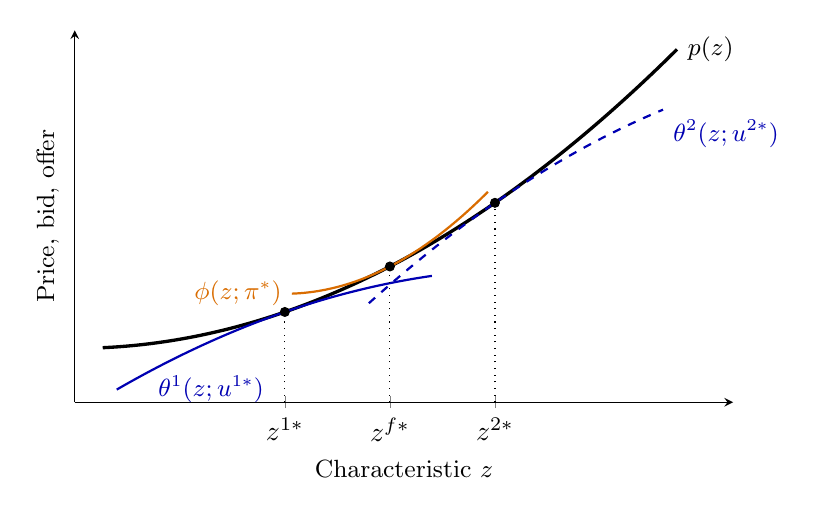
\begin{tikzpicture}
\begin{axis}[
  width=0.82\textwidth, height=0.52\textwidth,
  axis lines=left, xmin=0, xmax=4.7, ymin=0, ymax=6.9,
  xlabel={Characteristic $z$}, ylabel={Price, bid, offer},
  xtick={1.5,2.25,3}, xticklabels={$z^{1*}$, $z^{f*}$, $z^{2*}$},
  ytick=\empty, clip=false, every axis label/.append style={font=\small}]
  \addplot[domain=0.2:4.3, samples=120, very thick, black] {1+0.3*x^2}
    node[pos=1, right, font=\small] {$p(z)$};
  \addplot[domain=0.3:2.55, samples=80, thick, blue!70!black] {1.675+0.9*(x-1.5)-0.25*(x-1.5)^2};
  \node[anchor=east, font=\small, text=blue!70!black] at (axis cs:1.42,0.24) {$\theta^{1}(z; u^{1*})$};
  \addplot[domain=2.1:4.2, samples=80, thick, blue!70!black, dashed] {3.7+1.8*(x-3)-0.3*(x-3)^2}
    node[pos=1, below right, font=\small] {$\theta^{2}(z; u^{2*})$};
  \addplot[domain=1.55:2.95, samples=80, thick, orange!85!black] {2.51875+1.35*(x-2.25)+0.9*(x-2.25)^2}
    node[pos=0, left, font=\small] {$\phi(z; \pi^*)$};
  \addplot[only marks, mark=*, mark size=1.6pt] coordinates {(1.5,1.675) (2.25,2.51875) (3,3.7)};
  \draw[dotted] (axis cs:1.5,0) -- (axis cs:1.5,1.675);
  \draw[dotted] (axis cs:2.25,0) -- (axis cs:2.25,2.51875);
  \draw[dotted] (axis cs:3,0) -- (axis cs:3,3.7);
\end{axis}
\end{tikzpicture}
\caption{The hedonic price function $p(z)$. Consumer 1 and consumer 2 choose $z^{1*}$ and $z^{2*}$, where their bid curves
$\theta^{1}$ and $\theta^{2}$ (concave) touch $p(z)$ from below. A firm chooses $z^{f*}$, where its offer curve $\phi$ touches
$p(z)$ from above. At each traded bundle the slope of $p(z)$ equals the buyer's marginal willingness to pay and the seller's
marginal cost.}
\label{fig:06-hedonic}
\end{figure}

\casehead{Rosen's two-step procedure}
The model suggests two steps. First, regress the prices of products in a market on their characteristics with a flexible
functional form. This yields an estimate $\hat p(z)$ and implicit prices $\hat p_{z_k}(z_j)$ at each traded bundle. Second,
treat the implicit prices as observed marginal prices. Estimate the marginal bid functions $\hat p_{z_k}(z_j) =
F^k(z_j, Y_{1j})$, which depend on characteristics and buyer attributes $Y_{1j}$. Estimate them jointly with the marginal
offer functions $\hat p_{z_k}(z_j) = G^k(z_j, Y_{2j})$, which depend on seller attributes $Y_{2j}$.

\casehead{The identification critique}
The second step runs into two problems, which a one-characteristic example makes transparent. Let the price function be
quadratic,
\begin{equation*}
  p(z) = \pi_0 + \pi_1 z + \tfrac{1}{2}\pi_2 z^2 , \qquad \pi_2 > 0 ,
\end{equation*}
so the implicit price is $p_z(z) = \pi_1 + \pi_2 z$. The coefficients $\pi_0, \pi_1, \pi_2$ are unrelated to the profit $\pi$ of the offer function. Let consumer $i$'s marginal bid be linear,
\begin{equation*}
  \theta_z(z) = b_0 - b_1 z + b_2 Y_i + \eta_i , \qquad b_1 > 0 ,
\end{equation*}
where $Y_i$ is an observed attribute and $\eta_i$ an unobserved taste. The first-order condition $p_z(z_i) = \theta_z(z_i)$
gives
\begin{equation}\label{eq:06-rosen-choice}
  \pi_1 + \pi_2 z_i = b_0 - b_1 z_i + b_2 Y_i + \eta_i
  \quad\Longrightarrow\quad
  z_i = \frac{b_0 - \pi_1 + b_2 Y_i + \eta_i}{\pi_2 + b_1} .
\end{equation}

The first problem was raised by \citet{BrownRosen1982}. In one market the constructed implicit price $\pi_1 + \pi_2 z_i$ is
an exact linear function of $z_i$. Regressing it on $z_i$ and $Y_i$ fits perfectly with coefficients $(\pi_1, \pi_2, 0)$. The
second step merely reproduces the first-step price function and reveals nothing about the slope $-b_1$ of the marginal bid
curve. Identification requires restrictions that the data cannot supply in a single market, such as different functional
forms for the price function and the marginal bid function.

The second problem was stressed by \citet{Epple1987} and \citet{Bartik1987}. By \eqref{eq:06-rosen-choice}, the chosen
quantity $z_i$ rises with the unobserved taste $\eta_i$. Consumers who value the characteristic more buy more of it, and
along a nonlinear price function they also pay a higher implicit price. The regressor $z_i$ is correlated with the error of
the marginal bid equation. The consumer's own attributes are poor instruments, because they enter the bid function or may
correlate with unobserved tastes. A valid instrument must shift the price function that the consumer faces without
shifting tastes. Variation in $(\pi_1, \pi_2)$ across separate markets with the same distribution of tastes does this. In
market $m$ the first-order condition reads $\pi_{1m} + \pi_{2m} z_i = b_0 - b_1 z_i + b_2 Y_i + \eta_i$, and market indicators
identify $b_1$ through their effect on $z_i$.

\citet{EkelandHeckmanNesheim2004} show that the linear-quadratic structure behind the critique is special. Equilibrium
price functions are generically nonlinear, and with additive separability assumptions this nonlinearity can identify
preferences from a single market with one observed characteristic. Rosen's framework also connects to earlier sections.
Bresnahan's quality index $\delta(x) = \sqrt{\beta_0 + \sum_k x_k\beta_k}$ is read as a hedonic expansion path of
cost-minimizing characteristics, and his non-nested tests include a hedonic alternative (\cref{sec:06-bresnahan}).

\subsection{Bajari and Benkard: the model and the price function}\label{sec:06-bb-model}

\casehead{Motivation}
\citet[pp.~1--5]{BajariBenkard2005} give two reasons why hedonic models are rarely used in industrial organization. First,
Rosen assumes perfect competition and a continuum of products. Yet oligopoly is often the object of study, and oligopolistic
markets rarely contain more than a few hundred products. Under imperfect competition a hedonic price function need not
exist, and where it exists it is unlikely to be additively separable. Second, Rosen assumes that every characteristic is observed. In their data on personal computers,
357 of the 695 products are dominated. For each of them, another product is better in every observed characteristic and
cheaper. No hedonic model with full observability can rationalize positive demand for such products. Discrete choice models
avoid the problem through the shock $\epsilon_{ij}$. Bajari and Benkard instead add one characteristic that consumers see and
the econometrician does not.

They contrast their model with BLP-type models along the lines of \cref{sec:06-epsilon}. An i.i.d.\ shock makes the
characteristic space infinite dimensional. Together with the distributional assumptions, it typically produces demand curves
of hyperbolic shape that approach both axes. The hedonic model restricts demand only to slope downward, so the two models can
differ sharply when demand is predicted at prices outside the data.

\casehead{The model}
A product $j$ is a vector $(x_j, \xi_j)$, with $x_j \in \R^K$ observed by consumers and econometrician and a scalar $\xi_j$
observed by consumers only. Markets are indexed by $t \in \mathcal{T}$ and prices by $p_{jt}$. Consumer $i$ has utility
$u_i(x_j, \xi_j, c)$ over the product and a composite good $c \ge 0$ with price one. With income $y_i$, the consumer solves
(their eq.~1)
\begin{equation}\label{eq:06-bb-consumer}
  \max_{(j, c)}\; u_i(x_j, \xi_j, c) \quad\text{subject to}\quad p_{jt} + c \le y_i .
\end{equation}

\begin{assumption}[Bajari and Benkard, A1 to A3]\label{ass:06-bb}
For every consumer and market: (A1) $u_i$ is continuously differentiable and strictly increasing in $c$, with
$\frac{\partial u_i}{\partial c} \ge \underline{m} > 0$ for $c \in (0, y_i]$. (A2) $u_i$ is Lipschitz continuous in $(x_j,
\xi_j)$ with constant $L$. (A3) $u_i$ is strictly increasing in $\xi_j$.
\end{assumption}

We state the bounds $\underline{m}$ and $L$ as common to all consumers, which the Lipschitz property of the price function
requires. Assumption A3 is the strongest. It rules out satiation in the unobserved characteristic.

\begin{theorem}[Bajari and Benkard, Theorem~1]\label{thm:06-bb-pricefn}
Under \cref{ass:06-bb}, for any two products $j$ and $j'$ with positive demand in market $t$:
\begin{enumerate}[label=(\roman*)]
\item If $x_j = x_{j'}$ and $\xi_j = \xi_{j'}$, then $p_{jt} = p_{j't}$.
\item If $x_j = x_{j'}$ and $\xi_j > \xi_{j'}$, then $p_{jt} > p_{j't}$.
\item $|p_{jt} - p_{j't}| \le \bar L\bigl(\lVert x_j - x_{j'} \rVert + |\xi_j - \xi_{j'}|\bigr)$ with $\bar L = \frac{L}{\underline{m}}$.
\end{enumerate}
\end{theorem}

\begin{proof}
Each part shows that a violation would leave one of the two products with no buyers.

(i) Suppose $p_{jt} > p_{j't}$. A consumer who can afford $j$ gets the same product characteristics from $j'$ with more of the
composite good. By A1 she strictly prefers $j'$, so $j$ has no demand.

(ii) Suppose $p_{jt} \le p_{j't}$. For a consumer who can afford $j'$, A1 and then A3 give
\begin{equation*}
  u_i(x_j, \xi_j, y_i - p_{jt}) \ge u_i(x_j, \xi_j, y_i - p_{j't}) > u_i(x_j, \xi_{j'}, y_i - p_{j't}) ,
\end{equation*}
so $j'$ has no demand.

(iii) Let $d = \lVert x_j - x_{j'} \rVert + |\xi_j - \xi_{j'}|$ and suppose $p_{jt} - p_{j't} > \bar L d$. Take a consumer who can
afford $j$, so $y_i \ge p_{jt}$. Split the utility difference into a change in $c$ and a change in characteristics:
\begin{align*}
  u_i(x_{j'}, \xi_{j'}, y_i - p_{j't}) - u_i(x_j, \xi_j, y_i - p_{jt})
  &= \bigl[u_i(x_{j'}, \xi_{j'}, y_i - p_{j't}) - u_i(x_{j'}, \xi_{j'}, y_i - p_{jt})\bigr] \\
  &\quad + \bigl[u_i(x_{j'}, \xi_{j'}, y_i - p_{jt}) - u_i(x_j, \xi_j, y_i - p_{jt})\bigr] \\
  &\ge \underline{m}\,(p_{jt} - p_{j't}) - L d .
\end{align*}
The first bracket uses the mean value theorem and A1, and the second uses A2. The last expression exceeds $\underline{m} \bar L d -
L d = 0$. Every potential buyer of $j$ strictly prefers $j'$, so $j$ has no demand. Exchanging the roles of $j$ and $j'$
covers the other sign.
\end{proof}

The theorem uses only consumer optimization and the fact that consumers take prices as given. It places no restriction on
the supply side, so it holds under oligopoly and in static or dynamic equilibria. Its conclusions justify writing prices in
market $t$ as an equilibrium \emph{price function} $p_t(x, \xi)$ with $p_{jt} = p_t(x_j, \xi_j)$. Bajari and Benkard stress
what the function is not (their pp.~7--8). It is an equilibrium object that changes whenever any primitive changes: a new
product, a cost shock, a change in ownership. It does not predict the price of a product that is not on the market. It is
specific to each market. Even simple oligopoly models imply that it is nonlinear and not additively separable in $\xi$,
because markups depend on all characteristics. They therefore keep the general form.

\subsection{The first stage: the unobserved characteristic as a price quantile}\label{sec:06-bb-firststage}

The first stage recovers $\xi_j$ from prices. The unobserved characteristic has no natural units and is identified only up
to an increasing transformation. Bajari and Benkard normalize it to be uniform on $[0,1]$, which amounts to measuring it by
its own distribution function. Two further assumptions are needed.

\begin{assumption}[Bajari and Benkard, A4 and A5]\label{ass:06-bb-indep}
(A4) $\xi$ is independent of $x$. (A5) For every market $t$ and every $x$, $p_t(x, \cdot)$ is strictly increasing, with
$\frac{\partial p_t(x, \xi)}{\partial \xi} > \underline{\kappa}$ for all $(x, \xi)$ and some $\underline{\kappa} > 0$.
\end{assumption}

A4 strengthens the mean independence common in the literature. Because $\xi$ enters the price function
nonseparably, the model can still generate patterns that look like heteroskedasticity. Bajari and Benkard note that the
monotonicity in A5 follows from consumer preferences through \cref{thm:06-bb-pricefn}(ii). Let $F_{p_t \mid x = x_0}$ denote the distribution of
prices in market $t$ among products with observed characteristics $x_0$.

\begin{theorem}[Bajari and Benkard, Theorem~2]\label{thm:06-bb-xi}
Suppose prices are observed without error and A4 and A5 hold. Then for each market $t$ the price function $p_t$ is
identified within the class of price functions that are strictly increasing in $\xi$. The unobserved characteristics are
also identified:
\begin{equation}\label{eq:06-bb-xi}
  \xi_j = F_{p_t \mid x = x_j}(p_{jt}), \qquad p_t(x_0, e_0) = F^{-1}_{p_t \mid x = x_0}(e_0) .
\end{equation}
\end{theorem}

\begin{proof}
The argument is a chain of equalities.
\begin{align*}
  F_{p_t \mid x = x_j}(p_{jt}) &= \Pr\bigl(p_t(x, \xi) \le p_{jt} \mid x = x_j\bigr) && \text{(definition)} \\
  &= \Pr\bigl(\xi \le p_t^{-1}(x_j, p_{jt}) \mid x = x_j\bigr) && \text{($p_t(x_j, \cdot)$ strictly increasing)} \\
  &= \Pr\bigl(\xi \le p_t^{-1}(x_j, p_{jt})\bigr) && \text{(A4)} \\
  &= p_t^{-1}(x_j, p_{jt}) && \text{($\xi$ uniform on $[0,1]$)} \\
  &= \xi_j && \text{($p_{jt} = p_t(x_j, \xi_j)$).}
\end{align*}
Here $p_t^{-1}(x, \cdot)$ is the inverse of $p_t(x, \cdot)$. The same chain with $(x_0, p_t(x_0, e_0))$ in place of $(x_j,
p_{jt})$ gives $F_{p_t \mid x = x_0}(p_t(x_0, e_0)) = e_0$. Inverting this identity gives the second equation in
\eqref{eq:06-bb-xi}. Both objects are functions of the observable distribution of prices given characteristics, which
proves identification.
\end{proof}

The unobserved characteristic is the rank of a product's price among products with the same observed characteristics. A
computer priced at the 90th percentile among computers with identical observed specifications has $\xi = 0.9$. Identification
uses a single cross-section, so $\xi_j$ and its distribution may change over time. The first part of the argument follows
\citet{Matzkin2003}. If prices are measured with error, identification requires each product to be observed in many markets,
so that averaging removes the error (their Appendix~A, Theorem~6). The estimator replaces the conditional distribution with
a nonparametric estimate (their eq.~18):
\begin{equation}\label{eq:06-bb-xihat}
  \hat\xi_{jt} = \hat F_{p_t \mid x = x_j}(p_{jt}) .
\end{equation}
Kernel or series estimators can be used. In the application a local linear kernel estimator \citep{FanGijbels1996}
worked best.

Bajari and Benkard offer three alternatives to independence. Under \emph{options packages} (their Theorem~3), products are
grouped into models, such as a particular line of desktop computers, and an options package $x$ is chosen within a model.
All products of a model share the same $\xi$ (their A6), and a baseline package $\bar x$ is available for every model (their
A7). Normalizing $\xi$ given $x = \bar x$ to be uniform, $\xi_j$ is the price quantile of the baseline version of $j$'s model.
The approach is a nonparametric analog of fixed effects. It works in one cross-section even with measurement error, and it
is testable because many products share the same $\xi$.

Under a \emph{rich set of price functions} (their Theorem~4), some market has prices that depend on $\xi$ alone (their A8).
Packaged goods whose flavors all sell at the same price are an example. Prices weakly increase in $x$ and strictly increase
in $\xi$ in every market (their A9). With full support and products observed in many markets, these conditions identify the
ranking of the $\xi_j$. Finally, nonseparable nonparametric instrumental variables methods for triangular systems
\citep{ImbensNewey2009} could replace independence. They require instruments that determine the endogenous observed
characteristics yet are independent of $\xi$, and such instruments are hard to find in product markets.

\subsection{The second stage: preferences}\label{sec:06-bb-secondstage}

With $\xi$ recovered, Bajari and Benkard treat it as an observed characteristic. If demand were observed for every price
function, the results of \citet{MasColell1977} would recover preferences. Data are rarely that rich, and often each consumer
is observed once. Two cases arise.

\casehead{Continuous choice set}
Suppose utility is linear in the logarithms of the characteristics and in the composite good (their eq.~6):
\begin{equation}\label{eq:06-bb-u6}
  u_{ij} = \beta_{i1}\ln x_{1j} + \dots + \beta_{iK}\ln x_{Kj} + \beta_{i\xi}\ln \xi_j + c , \qquad c = y_i - p_t(x_j, \xi_j) .
\end{equation}
If the choice set is a continuum and the choice is interior, the consumer chooses $(x, \xi)$ on the price surface to maximize
\eqref{eq:06-bb-u6}. Differentiating with respect to $x_k$ and $\xi$ gives (their eqs.~7--8)
\begin{equation*}
  \frac{\beta_{ik}}{x_{kj}} = \frac{\partial p_t(x_j, \xi_j)}{\partial x_k}, \quad k = 1, \dots, K, \qquad
  \frac{\beta_{i\xi}}{\xi_j} = \frac{\partial p_t(x_j, \xi_j)}{\partial \xi} .
\end{equation*}
Solving for the tastes gives (their eqs.~9--10)
\begin{equation}\label{eq:06-bb-tastes}
  \beta_{ik} = x_{kj}\,\frac{\partial p_t(x_j, \xi_j)}{\partial x_k}, \qquad
  \beta_{i\xi} = \xi_j\,\frac{\partial p_t(x_j, \xi_j)}{\partial \xi} .
\end{equation}
A single observed choice therefore identifies a consumer's entire taste vector, given the price function and $\xi_j$. Each
taste is the implicit price of the characteristic times the chosen quantity, which is the consumer's willingness to pay, in
dollars, for a unit increase in the logarithm of the characteristic. Pooling consumers' choices traces out the population
distribution of tastes nonparametrically. The precision of these estimates depends only on the first-stage sample.

More generally, write $u_i(x, c) = u(x, y_i - p(x); \beta_i)$ with $\beta_i \in \R^B$ (their eq.~11). The first-order
conditions $\frac{\partial}{\partial x_k} u(x, y_i - p(x); \beta_i) = 0$ define the optimal choice $x(\beta)$. Implicit
differentiation gives $x'(\beta) = -[D_{xx}\bar u]^{-1} D_{x\beta}\bar u$, where $\bar u(x; \beta) = u(x, y_i - p(x); \beta)$
(their eqs.~12--14). Their Theorem~5 states that $\beta_i$ is locally identified when $x'(\beta)$ is locally positive or
negative definite, by the inverse function theorem. With as many taste parameters as characteristics ($B = K$) and $x'(\beta)$
definite everywhere on an open convex set, the map $x(\cdot)$ is one-to-one and tastes are globally identified
\citep{GaleNikaido1965}. One choice identifies at most $K$ random coefficients.

\casehead{Discrete choice set}
With finitely many products, utility maximization yields inequalities. If consumer $i$ chooses product $j$, then (their
eq.~15)
\begin{equation}\label{eq:06-bb-ineq}
  u(x_j, \xi_j, y_i - p_{jt}; \beta_i) \ge u(x_k, \xi_k, y_i - p_{kt}; \beta_i) \quad\text{for all } k \ne j ,
\end{equation}
so $\beta_i$ lies in the \emph{revealed preference set} $A_{ij} = \{\beta : \text{\eqref{eq:06-bb-ineq} holds}\}$ (their
eq.~16). The set typically contains more than one point, so individual tastes are not identified. It can still be small when
the choice set is rich. If every characteristic is continuous and the products fill a compact set, the sets shrink to points as the number
of products grows (their Appendix~B, Theorem~8). Their rate argument is simple. In their Appendix~B, utility
$u(x_j, p_j; \beta_i)$ does not depend on income, and there is no outside option. Each set then depends only on the
product chosen, and the sets for the $J$ products partition the bounded parameter space $\mathcal{B}$. Their average
Lebesgue measure is therefore $\frac{m(\mathcal{B})}{J}$. An outside option would add one more set and leave the rate
unchanged. Consumers who buy
nothing are treated as buying a bundle with zero characteristics at zero price (their eq.~17):
\begin{equation*}
  u(0, 0, y_i; \beta_i) \ge u(x_k, \xi_k, y_i - p_{kt}; \beta_i) \quad\text{for all } k .
\end{equation*}
These conditions are only inequalities, so the tastes of non-purchasers are not point identified even with a continuous
product space.

The sets $A_{ij}$ deliver bounds on the population distribution of tastes. Let $\mathcal{B}(\bar\beta) = \{\beta : \beta \le
\bar\beta\}$. The share of consumers whose whole set $A_{ij}$ lies in $\mathcal{B}(\bar\beta)$ is a lower bound for the taste
distribution function at $\bar\beta$. The share whose set meets $\mathcal{B}(\bar\beta)$ is an upper bound. When utility is
quasi-linear, as in \eqref{eq:06-bb-u6}, income cancels from \eqref{eq:06-bb-ineq}. All buyers of product $j$ then share one
set $A_j$, and product-level quantities suffice for estimation.

\casehead{A Bayesian point estimate and the Gibbs sampler}
For a point estimate, Bajari and Benkard turn the inequalities into a likelihood. Consumer $i$ with tastes $\beta_i$ chooses
$j$ with likelihood (their eq.~21)
\begin{equation}\label{eq:06-bb-lik}
  L(j \mid x, y_i, \beta_i) = \indic\bigl\{u(x_j, y_i - p_j; \beta_i) \ge u(x_k, y_i - p_k; \beta_i) \text{ for all } k \ne j\bigr\} ,
\end{equation}
where $x_j$ now includes $\xi_j$. With a uniform prior on a box $\mathcal{B}$ that contains every $A_{ij}$, the posterior
$\pi(\beta_i \mid j) \propto \indic\{\beta_i \in \mathcal{B}\}\, L(j \mid x, y_i, \beta_i)$ is uniform on $A_{ij}$ (their
eq.~22).

Sampling from a uniform distribution on a set defined by many inequalities is easy coordinate by coordinate. In model
\eqref{eq:06-bb-u6}, choice of $j$ requires, for every $k \ne j$ (their eq.~29),
\begin{equation*}
  \sum_{l} \beta_{il}\ln x_{lj} + y_i - p_j \ge \sum_{l} \beta_{il}\ln x_{lk} + y_i - p_k .
\end{equation*}
Collecting the terms in $\beta_{i1}$ gives
\begin{equation*}
  \beta_{i1}\,(\ln x_{1j} - \ln x_{1k}) \ge \sum_{l \ne 1} \beta_{il}(\ln x_{lk} - \ln x_{lj}) + (p_j - p_k) .
\end{equation*}
Define the ratio
\begin{equation}\label{eq:06-bb-ratio}
  R_k(\beta_{i,-1}) = \frac{\sum_{l \ne 1} \beta_{il}(\ln x_{lk} - \ln x_{lj}) + (p_j - p_k)}{\ln x_{1j} - \ln x_{1k}} .
\end{equation}
If $x_{1j} > x_{1k}$, the denominator is positive and the inequality reads $\beta_{i1} \ge R_k$. If $x_{1j} < x_{1k}$,
dividing by a negative number flips it to $\beta_{i1} \le R_k$. If $x_{1j} = x_{1k}$, the inequality does not involve
$\beta_{i1}$. Given the other coordinates, $\beta_{i1}$ is therefore uniform on $[\beta_{1,\min}, \beta_{1,\max}]$ with
(their eqs.~32--33)\footnote{The working paper prints the price term in eqs.~30--33 as $(y_i - p_j) - (y_i - p_k)$, which
has the opposite sign. The expression here follows from their eq.~29.}
\begin{equation}\label{eq:06-bb-bounds}
  \beta_{1,\min} = \max\Bigl\{\underline b_1,\ \max_{k : x_{1j} > x_{1k}} R_k(\beta_{i,-1})\Bigr\}, \qquad
  \beta_{1,\max} = \min\Bigl\{\bar b_1,\ \min_{k : x_{1j} < x_{1k}} R_k(\beta_{i,-1})\Bigr\},
\end{equation}
where $[\underline b_1, \bar b_1]$ is the range of the first coordinate in the prior box. The other coordinates are
handled in the same way. The sampler proceeds as follows.
\begin{enumerate}
\item Start from a point $\beta_i^{(0)}$ in $A_{ij}$. Bajari and Benkard use the tastes implied by the continuous-case
formulas \eqref{eq:06-bb-tastes} and search nearby when that point violates an inequality.
\item Given $\beta_i^{(s)}$, draw $\beta_{i1}^{(s+1)}$ from the uniform distribution on $[\beta_{1,\min}, \beta_{1,\max}]$
computed at the current values of the other coordinates.
\item Draw each remaining coordinate $l = 2, \dots, K$ in the same way, conditioning on the most recent values of the others.
\item Repeat, discarding an initial set of draws.
\end{enumerate}
Each inequality is linear in $\beta_i$, so $A_{ij}$ is an intersection of half-spaces. It is therefore convex, hence
connected, and standard sufficient conditions for convergence of the sampler hold (their footnote~8). The distribution
function of tastes is estimated by the frequency of draws below each point (their eq.~34),
\begin{equation}\label{eq:06-bb-cdf}
  \hat F(\bar\beta_1, \dots, \bar\beta_K) = \frac{1}{S}\sum_{s=1}^{S} \indic\bigl\{\beta^{(s)}_1 \le \bar\beta_1, \dots, \beta^{(s)}_K \le \bar\beta_K\bigr\} ,
\end{equation}
with draws pooled across consumers. The uniform prior selects one distribution among the many consistent with the data. The
sampler extends to repeated choices, which add inequalities, and to estimation error in $\xi$, by drawing $\xi$ from its
sampling distribution before each run.

\casehead{When independence fails}
If $\xi$ is locally positively correlated with some observed characteristic, the first stage attributes part of the price
effect of $\xi$ to that characteristic. Its implicit price is biased upward and the implicit price of $\xi$ downward. Through
\eqref{eq:06-bb-tastes} the estimated tastes inherit the same biases. Because a product is a bundle of both characteristics,
the biases partly offset in the demand for products. Bajari and Benkard report that they cancel exactly with linear utility
and a linear price function.

\subsection{Application: personal computers, December 1999}\label{sec:06-bb-pc}

\casehead{Data}
The data come from the PC Data Retail Hardware Monthly Report. They contain quantities, average prices and characteristics of
desktop computers for 29 months. The analysis concentrates on December 1999, with 695 models, a cross-section in which
traditional demand methods typically struggle. The data reportedly cover about 75 percent of U.S.\ retail computer sales.
Processor dummies are replaced by a CPU benchmark score, which a regression on chip speed interacted with chip dummies explains
with an $R^2$ of 0.999. The final data contain 19 characteristics. The three main continuous characteristics are the benchmark, RAM
and hard drive capacity. Following their Table~1, the others are MMX, SCSI, CD-ROM, DVD, a network card, a monitor dummy, monitor size, a zip
drive, desktop versus tower, refurbished and no modem. Five operating-system dummies complete the list, one of which is
omitted in the regression. With all characteristics treated as observed, 357 of the 695 products are dominated.
\Cref{tab:06-bb-data} reproduces selected rows of their Table~1, including an OLS hedonic regression.

\begin{table}[htbp]
\centering
\caption{Personal computers, December 1999: summary statistics and a linear hedonic regression}
\label{tab:06-bb-data}
\small
\begin{tabular}{@{}lrrrrr@{}}
\toprule
Variable & Mean & S.D. & Min & Max & OLS coefficient \\
\midrule
CPU benchmark          & 1354.5 & 362.3 & 516 & 2544 & 0.836 \\
RAM (MB)               & 74.0 & 35.1 & 16 & 256 & 3.010 \\
Hard drive (MB)        & 9276.8 & 4850.3 & 2100 & 40000 & 0.008 \\
MMX                    & 0.64 & 0.48 & 0 & 1 & $-56.971$ \\
SCSI                   & 0.01 & 0.08 & 0 & 1 & 310.747 \\
CD-ROM                 & 0.67 & 0.47 & 0 & 1 & 26.478 \\
DVD                    & 0.14 & 0.35 & 0 & 1 & 32.213 \\
Monitor included       & 0.31 & 0.46 & 0 & 1 & 29.625 \\
Monitor size           & 0.75 & 3.27 & 0 & 15 & 22.822 \\
Desktop (not tower)    & 0.17 & 0.37 & 0 & 1 & 25.611 \\
Refurbished            & 0.09 & 0.28 & 0 & 1 & $-144.314$ \\
No modem               & 0.55 & 0.50 & 0 & 1 & 145.169 \\
\midrule
Constant               & & & & & $-590.2$ \\
$R^2$                  & & & & & 0.79 \\
$N$                    & & & & & 695 \\
\bottomrule
\end{tabular}

\smallskip
\begin{minipage}{0.85\textwidth}
\footnotesize Source: \citet{BajariBenkard2005}, Table~1 (working-paper version). The dependent variable of the OLS
regression is price in dollars. Rows not shown are the network card, zip drive and four operating-system dummies (Windows NT
4.0, Windows NT, Windows 98, Windows 95, with Windows 3.1 omitted). The paper reports no standard errors for this regression.
\end{minipage}
\end{table}

\casehead{First stage}
A nonparametric estimator in 19 dimensions is impractical, so the first stage treats three continuous characteristics
nonparametrically: CPU benchmark, RAM and hard drive. The price function is assumed additively separable in the other 16, with
coefficients fixed at the OLS values of \cref{tab:06-bb-data}. Bajari and Benkard argue that many of these are peripherals that
can be bought and sold separately, so arbitrage limits nonseparability. The estimator is \eqref{eq:06-bb-xihat} with a local
linear kernel and a normal kernel. Bandwidths were chosen by eye, which oversmooths relative to the mean-squared-error optimum.
Smooth estimates help because derivatives of the price function supply starting values for the sampler. With a finite product
space, only the $\hat\xi_j$ are needed for the demand system itself.

The unobserved characteristics are precisely estimated (their Table~2). Asymptotic standard errors average 0.010, have median
0.009, and are below 0.018 for 95 percent of products, with a maximum of 0.104. Bootstrap standard errors, from 1,000 samples
drawn with i.i.d.\ sampling of products, average 0.012, have 95th percentile 0.022 and maximum 0.121. For 508 of the 695
products the bootstrap standard error exceeds the asymptotic one. Two features explain the precision. A quantile is easier to
estimate than a density, and the characteristic space is densely filled, so almost every product has close neighbors. The
estimated bias was small and barely changed the ranking of the $\hat\xi_j$, so it was left out.

\casehead{Second stage}
The demand system uses all 19 observed characteristics and $\xi$. Utility is quasi-linear, linear in the logarithms of CPU
benchmark, hard drive, RAM and $\xi$, and linear in the other characteristics and in price. The $\hat\xi_j$ were rescaled so
that budget sets are convex, and other normalizations changed the results little. After discarding initial draws, the sampler
produced 1,000 taste draws per product, a total of 695,000 twenty-dimensional draws. These were reweighted by each product's
sales. Including the initial draws, the computation took about an hour on their Sun Ultra 60 workstation.

The estimated willingness-to-pay distributions (their Figures~1--5) look roughly lognormal except for the CPU benchmark. The
modal marginal willingness to pay is between \$1 and \$2 per megabyte of RAM and about 1.25 cents per megabyte of hard drive.
The data are informative even about the taste for SCSI, a dummy characteristic, because extreme values of one coefficient
require extreme values of others to rationalize a choice. Tastes are strongly positively correlated (their Table~3). The
correlation between the CPU and SCSI coefficients is 0.694, between RAM and hard drive 0.533, and between CPU and RAM 0.510. The
taste for $\xi$ correlates positively with every other taste, from 0.351 with hard drive to 0.477 with RAM. This arises even
though $\xi$ was assumed independent of $x$ in the first stage.

\casehead{Elasticities}
Aggregating the taste draws gives demand curves and elasticities for every product. With all 695 products the median
own-price elasticity $\varepsilon_{jj}$ was about $-100$. Bajari and Benkard read this as a rejection of perfect information. With 695 products,
neighbors are close in price and characteristics, so a fully informed consumer would switch at a tiny price change. Real
consumers search and consider only a handful of products. They therefore re-estimated the model with only the 24 products that
sold at least 5,000 units, a minimum share of 0.75 percent. These products account for 72 percent of sales. Own-price
elasticities then range from $-4$ to $-72$, with a median of $-11$. They caution that the selection retained similar
best-selling products, so these elasticities may still be too large in magnitude.

\begin{table}[htbp]
\centering
\caption{The five best-selling computers in December 1999 and their estimated price elasticities}
\label{tab:06-bb-elast}
\small
\begin{tabular}{@{}llrrrr@{}}
\multicolumn{6}{@{}l}{\emph{Panel A. Characteristics (Table 4)}} \\
\toprule
Model & CPU (benchmark) & RAM & Hard drive & Price (\$) & Sales \\
\midrule
HP Pavilion 6535      & Intel Celeron 466 MHz (1281) & 64 MB & 8.4 GB  & 590 & 71,199 \\
Compaq Presario 5441  & AMD K6-2 475 MHz (1076)      & 64 MB & 8.0 GB  & 540 & 54,449 \\
Compaq Presario 5461  & AMD K6-2 500 MHz (1115)      & 64 MB & 10.0 GB & 727 & 43,029 \\
E-Machines eTower 433 & Celeron 433 MHz (1167)       & 32 MB & 4.3 GB  & 471 & 40,399 \\
HP Pavilion 6545C     & Celeron 500 MHz (1398)       & 64 MB & 13.0 GB & 858 & 34,198 \\
\bottomrule
\end{tabular}

\bigskip
\begin{tabular}{@{}lrrrrr@{}}
\multicolumn{6}{@{}l}{\emph{Panel B. Matrix of price elasticities (Table 5)}} \\
\toprule
 & HP6535 & Compaq5441 & Compaq5461 & E-Machines & HP6545C \\
\midrule
HP6535      & $-4.14$ & 0.12    & 0.00    & 0.43     & 0.28 \\
Compaq5441  & 0.17    & $-5.95$ & 2.98    & 0.73     & 0.55 \\
Compaq5461  & 0.00    & 2.80    & $-8.00$ & 0.85     & 0.11 \\
E-Machines  & 0.61    & 0.69    & 0.91    & $-10.65$ & 0.66 \\
HP6545C     & 0.70    & 0.86    & 0.18    & 1.02     & $-4.46$ \\
\bottomrule
\end{tabular}

\smallskip
\begin{minipage}{0.92\textwidth}
\footnotesize Source: \citet{BajariBenkard2005}, Tables~4 and~5 (working-paper version). Table~4 of the paper prints the
processor as ``AMD A6-2''. Panel A corrects it to the AMD K6-2 chip. Elasticities come from the model estimated on the 24 products
selling at least 5,000 units. The paper does not state whether rows or columns index the product whose price changes.
\end{minipage}
\end{table}

\Cref{tab:06-bb-elast} shows the five best sellers and their elasticity matrix. Two features stand out. The most similar
products substitute most, as the two Compaq models do (2.98 and 2.80). Some cross elasticities are exactly zero: the HP6535 and
the Compaq5461 do not substitute at all, presumably because other products lie between them in characteristic space. A model with
an i.i.d.\ shock cannot produce a zero cross elasticity, since every product keeps some buyers who rank it second.

\begin{figure}[htbp]
\centering
\begin{subfigure}[t]{0.8\textwidth}
\centering
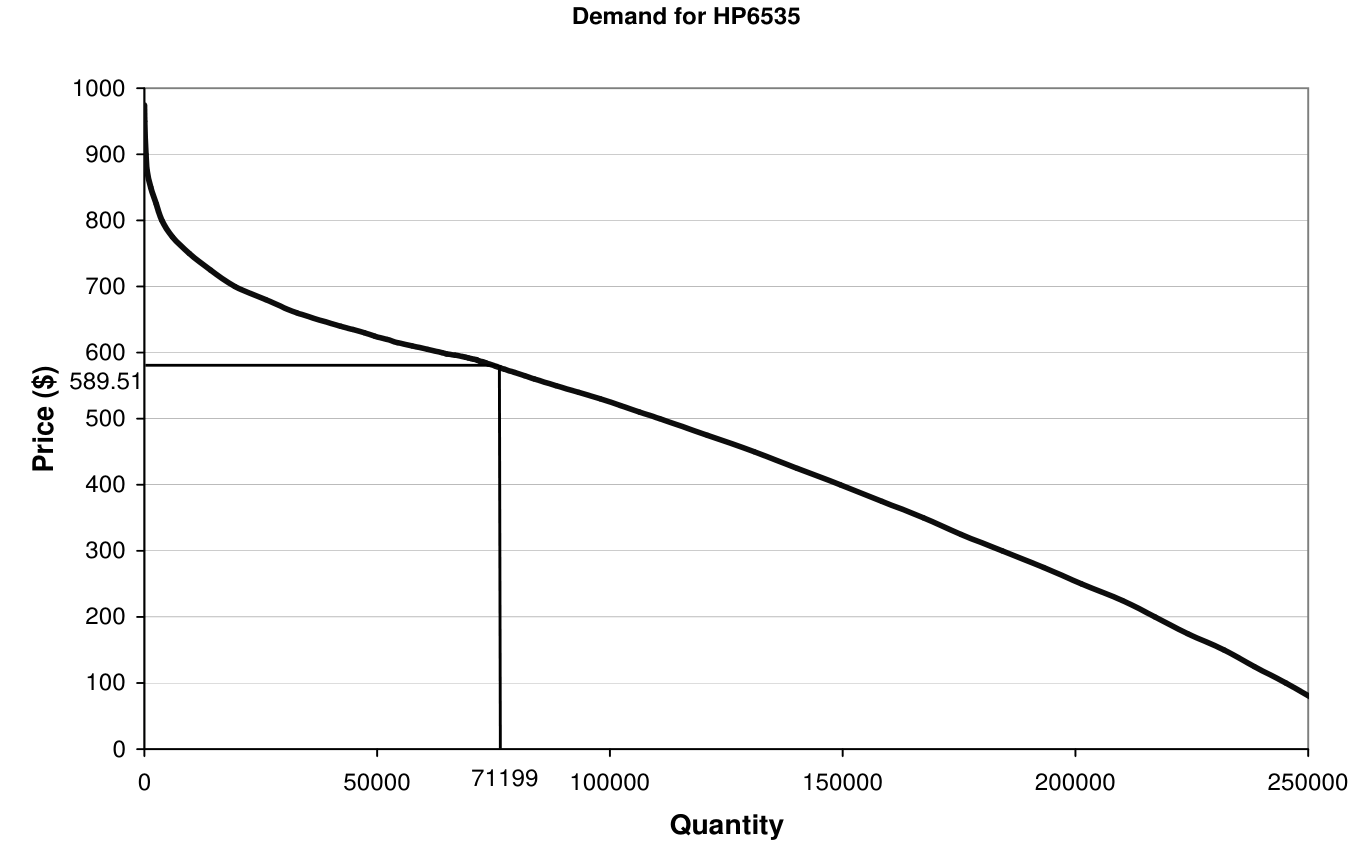
\includegraphics[width=\textwidth]{figures/ch06/bb_fig6_demand.png}
\caption{Estimated demand for the HP Pavilion 6535}
\end{subfigure}\par\medskip
\begin{subfigure}[t]{0.8\textwidth}
\centering
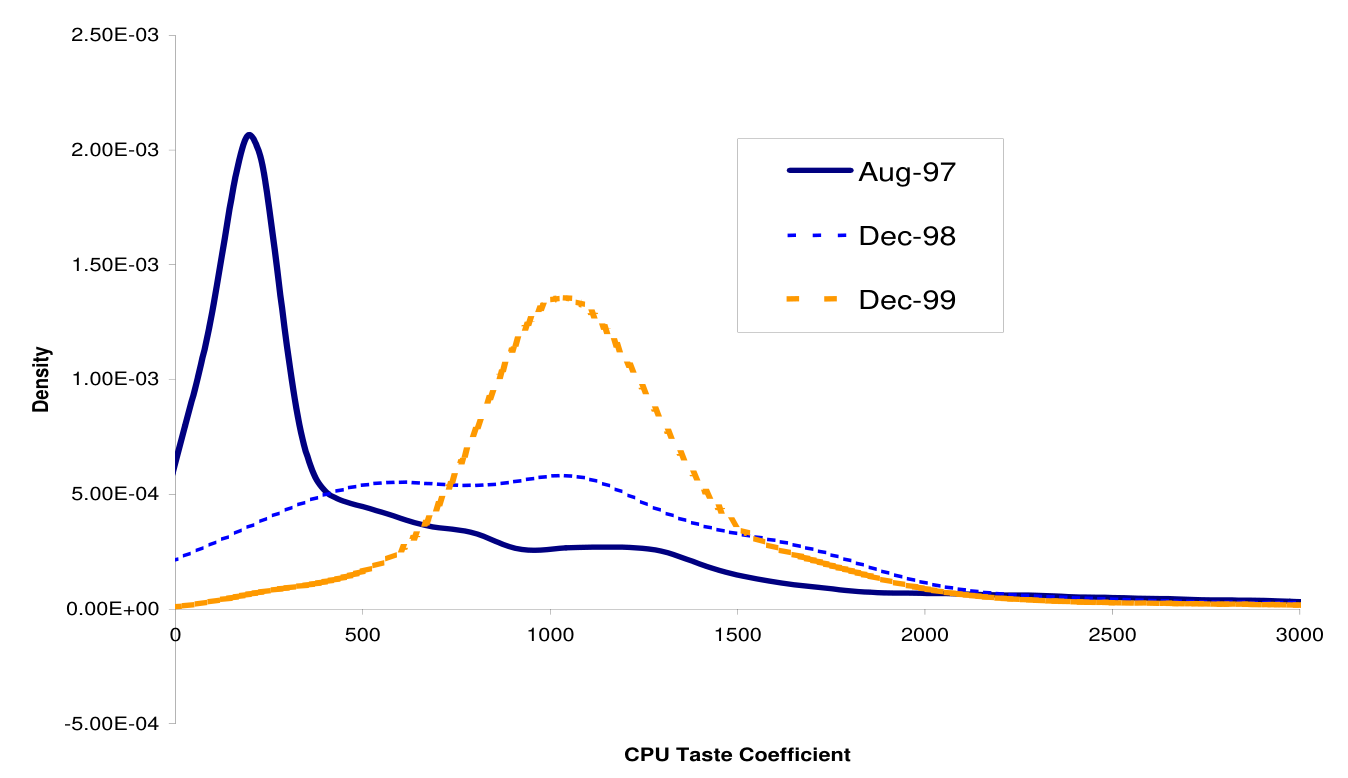
\includegraphics[width=\textwidth]{figures/ch06/bb_fig7_cputaste.png}
\caption{Estimated density of the taste for CPU}
\end{subfigure}
\caption{Panel (a) shows the estimated demand curve of the HP Pavilion 6535, with the observed price (\$589.51) and quantity
(71,199) marked. Panel (b) shows the estimated distribution of the CPU taste coefficient in August 1997, December 1998 and
December 1999. Source: Bajari and Benkard (2005), Figures~6 and~7 (working-paper version).}
\label{fig:06-bb-demand}
\end{figure}

Panel (a) of \cref{fig:06-bb-demand} shows the estimated demand curve for the HP6535. It is steep at high prices, flat near the
observed price and steep again at low prices. A small group of consumers strongly prefers this model, which explains the steep
upper part. Near the observed price many consumers would switch to neighboring products for little compensation, which flattens
the curve. At low prices the product already has a large share and few consumers remain to be won. Utility maximization forces
the curve to slope down, but nothing else restricts its shape. Bajari and Benkard contrast it with the curves of standard
discrete choice models, which approach both axes, and with those of multi-stage budgeting models, which are typically quadratic.

Panel (b) shows estimates from other months of the data. The distribution of the CPU taste shifts up sharply between August
1997 and December 1999. In the intermediate period it has markedly higher variance. Bajari and Benkard attribute the shift to
complementarity with the rapidly growing use of the internet. The evidence suggests that the common assumption of a taste
distribution that is constant over time would fail in this industry.

\casehead{Assessment}
The hedonic approach estimates the distribution of a twenty-dimensional taste vector nonparametrically. It allows demand
curves of any downward-sloping shape and exact zeros in the matrix of cross elasticities. It identifies the unobserved
characteristic from a single cross-section without instruments for price, because price is a function of $(x, \xi)$ and $\xi$
is recovered from the price distribution itself. Its costs are equally clear. The first stage needs many products per market
and full independence of $\xi$ from $x$, stronger than the mean independence that BLP-type estimators impose relative to
their instruments. \citet[p.~35]{AckerbergEtAl2007} stress that the consistency of the first stage rests on asymptotics in
the number of products. Products must eventually ``fill up'' the characteristic space, so that every product has others
with observed characteristics arbitrarily close to its own. They add that experience is still too limited to know what
``many'' products means here. The unobservable is single and vertical. Consumers are assumed fully informed, which the elasticities with
695 products reject.

The comparison with \citet{BerryPakes2007} is instructive. Both papers drop the idiosyncratic shock and keep one vertical
unobservable. Berry and Pakes keep a parametric taste distribution, invert market shares for $\xi$ and use instruments for price,
following \citet{BerryLevinsohnPakes1995}. Bajari and Benkard recover $\xi$ from prices and use revealed preference to recover a
nonparametric taste distribution. In both, many close substitutes produce very large elasticities. This suggests that in models
with tastes for products the shock $\epsilon_{ij}$ partly stands in for frictions such as limited information and search, which
pure characteristics models must then model explicitly. The random coefficients logit of \cref{ch:blp} remains the workhorse,
and the models of this section and the last are the natural checks on what its shock assumes.
